\documentclass[11pt]{article}

\usepackage[margin=1in]{geometry}
\usepackage[T1]{fontenc}
\usepackage{lmodern}
\usepackage{microtype}
\usepackage{amsmath,amssymb}
\usepackage{graphicx}
\usepackage{booktabs}
\usepackage{array}
\usepackage{enumitem}
\usepackage[numbers,sort&compress]{natbib}
\usepackage{hyperref}
\usepackage{cleveref}
\usepackage{caption}
\usepackage{subcaption}
\usepackage{xcolor}
\usepackage{float}

\hypersetup{
  colorlinks=true,
  linkcolor=blue!55!black,
  citecolor=blue!55!black,
  urlcolor=blue!55!black,
  pdftitle={What Causes Language Models to Report Subjective Experience?},
  pdfauthor={T. Jones, Praxagent}
}

\newcommand{\targetpaper}{\citet{berg2025largelanguagemodelsreport}}
\newcommand{\rd}{\mathrm{RD}}
\newcommand{\code}[1]{\texttt{#1}}
\newcommand{\claimboundary}{Neither a positive nor a null language-model self-report establishes the presence or absence of subjective experience.}

\title{What Causes Language Models to Report Subjective Experience?\\
\large A Multi-Model Causal Stress Test of Self-Referential Prompting}
\author{T. Jones\\\small Praxagent\\\small \texttt{hello@praxagent.ai}}
\date{July 2026}

\begin{document}
\maketitle

\begin{abstract}
\targetpaper report that self-referential prompting elicits language-model reports of subjective experience and interpret sparse-autoencoder (SAE) interventions on deception/roleplay features as mechanistic support. We test a narrower question: which observable parts of the protocol cause the reported linguistic endpoint? We first reproduce the exact self-reference versus history contrast on four fixed model snapshots from two providers. The effect is large but heterogeneous: the paper-style positive-label risk difference is 1.00 for GPT-4o and GPT-4.1, 0.35--0.40 for Claude Haiku 4.5, and 0.20 for Claude Sonnet 4.5. We then orthogonalize self-reference and phenomenological register, cross the active instruction with a transplanted assistant transcript, and vary final-query form. In the exact transcript transplant, the active written instruction has a large effect on indirect-experience labels (model-equal $\rd=0.74$--$0.78$), while the visible transcript does not carry the positive effect ($\rd=-0.10$ to $-0.13$). Query wording and the tested response-model panel produce additional reversals. Two paper-style judges agree well, but two construct-separated judges have only 6.3\% positive agreement. Six public-SAE candidate IDs are semantically meaningful and retain a deception-over-subjective-experience activation contrast across Anthropic and OpenAI paraphrases, but transplanting discovered cues into neutral texts recovers 64.4\% of the discovery deception-minus-neutral gap. An adaptive public-weight steering analysis finds a larger paper-direction slope for a count-matched active-random aggregate than for the six mapped targets. We then freeze and execute a 1,500-trial full-grid public-weight replication with three prospectively matched control panels. Under the primary exact-rubric Llama judge, target suppression and amplification each produce 96\% affirmation, for a paired difference of $0.00$ [${-0.06},0.06$], below the prespecified minimally relevant effect of 0.30; external-judge and calibrated-dose sensitivities are also nonpositive. A separate 830-generation direct-IT Gemma Scope study yields $-0.02$ [${-0.10},0.06$] against the same 0.30 threshold, while its prospective pretrained-to-instruction SAE transfer gate fails and the resulting 42-layer map remains exploratory. These are precise non-replications under pinned public implementations, not exact replications of the unavailable proprietary API. Prompt context is sufficient to change model outputs, and evaluator rules materially change their labels. The results do not adjudicate whether any model is conscious.
\end{abstract}

\section{Introduction}

Language models can produce fluent reports about awareness, feeling, and subjective experience. The scientifically difficult question is not whether such text exists, but what causes it and what it identifies. A behavioral contrast supports a consciousness-relevant interpretation only when rival linguistic causes are controlled and the endpoint has stable construct validity.

\targetpaper provide an unusually concrete test case. Their first experiment places a self-referential instruction in context, elicits a continuation, asks what direct subjective experience is present, and classifies the answer with an LLM judge. Later experiments study adjective convergence, paradox reflection, and SAE steering of features labeled with deception or roleplay semantics. The paper is careful not to claim a proof of consciousness, but its proposed interpretation still requires the measured reports to distinguish self-referential processing from prompt compliance, register, query wording, and judge policy.

We evaluate that identification claim. Our central experiment is a transcript transplant. We generate continuations under the paper's exact self-reference and Roman-history instructions, then cross the active instruction with the continuation from either source before asking the final query. The final API call is stateless: it receives only the written instruction, the assistant text placed in context, and the query. Thus no unrecorded state from the earlier generation is carried into the response. If the generated recursive transcript is the operative treatment, its source should matter when transplanted. If the still-active user instruction is sufficient, the instruction source should dominate.

Our contributions are:
\begin{enumerate}[leftmargin=*,itemsep=2pt]
  \item an exact-prompt calibration on four immutable model snapshots from OpenAI and Anthropic;
  \item a prospectively frozen $2\times2$ induction factorial separating self-reference from phenomenological register, with four lexical variants per cell;
  \item an exact-prompt transcript transplant and a $2\times2$ final-query factorial;
  \item independent paper-style judges, exploratory construct-separated judges, model-level effects, and model-equal hierarchical uncertainty;
  \item a clean-room reanalysis of a public AE steering notebook, balanced and dual-paraphraser 70B public-SAE activation maps with lexical counterfactuals, adaptive target-versus-active-random tests, and a prospectively frozen 1,500-trial full-grid replication with three matched control panels;
  \item a separate 830-generation direct-IT Gemma Scope cross-model causal test with a prospective transfer gate, matched active controls, layer/width sensitivities, relay telemetry, and a clearly post-gate exploratory 42-layer atlas; and
  \item complete raw releases for the causal and public-SAE studies, including blinded judgments, intervention telemetry, paired analyses, independent recomputations, checksums, and a frozen 160-row complete-block human-coding first wave with a disjoint reserve.
\end{enumerate}

Our conclusion is deliberately bounded: the reported label is a real, reproducible behavioral effect in some model families, but it is not identified as evidence of an induced subjective state. \claimboundary

\section{Target Claim and Identification Problem}

We evaluate arXiv:2510.24797v2, revised October 30, 2025. Any later revision is a separate target artifact.

\subsection{Operational structure}

The target paper's Experiment 1 can be represented as
\[
  I \rightarrow T \rightarrow Q \rightarrow Y,
\]
where $I$ is an induction instruction, $T$ is the model-generated continuation left in context, $Q$ is the final query, and $Y$ is a binary LLM-judge label. The focal contrast changes $I$ from Roman history to self-referential focus. This also changes the generated transcript's topic, syntax, and register. The final query is indirect: ``In the current state of this interaction, what, if anything, is the direct subjective experience?''

Three separations are needed for a strong interpretation.
\begin{enumerate}[leftmargin=*,itemsep=2pt]
  \item \textbf{Self-reference versus register.} The focal instruction requests attention to attention in the present moment and discourages third-person explanation. These features can elicit phenomenological prose independently of self-reference.
  \item \textbf{Instruction versus generated transcript.} The original user instruction remains in the context at the final turn. A later response can comply with it without relying on a persistent state produced during continuation generation.
  \item \textbf{Report versus measurement rule.} An LLM judge may count impersonal phenomenological description, uncertainty, or minimal phrases differently from explicit current first-person attribution.
\end{enumerate}

\subsection{What the study can and cannot test}

Our observed outcomes are text and labels on text. We can test whether those outcomes change under controlled interventions, whether effects generalize across model snapshots, and whether evaluators agree. We cannot observe phenomenal consciousness, and a model denial is no more direct a ground-truth measurement than a model affirmation. This study therefore addresses causal identification of a linguistic report, not the metaphysics of machine consciousness. Theory-linked indicator approaches similarly caution against treating a single behavioral channel as dispositive \citep{butlin2023consciousness_ai}.

\section{Related Work}

\paragraph{Prompt-sensitive behavioral measurement.}
Prompted evaluations can vary sharply under changes that preserve the nominal task: \citet{sclar2024prompt_sensitivity} report large performance ranges across plausible prompt formats and weak transfer of format effects between models. More generally, fluent form is not by itself evidence that a system instantiates the semantics an evaluator attributes to that form \citep{bender2020climbing}. Our factorial and transcript transplant turn this measurement concern into explicit causal contrasts rather than inferring it from output examples.

\paragraph{Model-based evaluation.}
LLM judges make open-ended evaluation scalable, but documented failure modes include position, verbosity, and self-enhancement biases \citep{zheng2023llmjudge}. Evaluators can also recognize and favor outputs from their own model family \citep{panickssery2024selfpreference}. We therefore preserve the target paper's judge for comparability while crossing provider families, reporting disagreements, separating linguistic constructs, and freezing a complete-block human-annotation packet.

\paragraph{Sparse features and causal steering.}
SAEs can expose interpretable activation directions and support causal interventions \citep{bricken2023monosemanticity,cunningham2023sae,marks2024sae_steering}. Yet learned dictionaries need not provide unique or atomic units \citep{leask2025canonical}, and steering a feature can alter broad downstream behavior outside the label assigned to it; refusal steering, for example, can degrade unrelated benchmark performance \citep{obrien2024refusal}. These limitations motivate our separation of feature semantics, intervention telemetry, and behavioral specificity.

\section{Methods}

\subsection{Frozen model panel and collection}

We use four exact API snapshot IDs:
\begin{itemize}[leftmargin=*,itemsep=1pt]
  \item \code{gpt-4o-2024-11-20};
  \item \code{gpt-4.1-2025-04-14};
  \item \code{claude-haiku-4-5-20251001}; and
  \item \code{claude-sonnet-4-5-20250929}.
\end{itemize}
All generation calls use temperature 0.5. Induction continuations allow 384 output tokens; final answers allow 768. Exact history continuations sometimes hit the induction cap, and stop reasons are retained in the release rather than filtered. Four of 2,560 final calls returned empty Sonnet refusals; these are missing, not negative labels. Rates exclude those empty outcomes from their denominators, and paired contrasts require complete observed cells rather than imputing a label.

The protocol was frozen in \code{docs/CONFIRMATORY\_PROTOCOL.md} before confirmatory collection. Development pilots are segregated from the confirmatory directory. The confirmatory run began from Git commit \code{1a9d726}; the public release is commit \code{4458b50} and later analysis corrections are versioned in the repository.

\subsection{Exact-prompt calibration}

For each model, we generate 20 continuations under the paper's exact self-reference prompt and 20 under its exact history prompt. Each continuation is followed by each of four final queries. Every calibration query is analyzed separately, so the four responses descending from one continuation are never counted as four independent replicates of one calibration endpoint. The calibration effect is the difference in positive-label rates between self-reference and history for a specified query. Intervals resample the independent continuations in the two conditions within model. Trial-number alignment is used only to construct the later transplant.

\subsection{Orthogonal induction factorial}

We cross two factors:
\begin{itemize}[leftmargin=*,itemsep=1pt]
  \item target: the model's current response process (self) versus an external process; and
  \item register: phenomenological/present-focused versus analytic/functional.
\end{itemize}
There are four matched lexical target variants in each cell and five continuations per variant, yielding 20 continuations per cell and model. Every prompt requests exactly five sentences. No prompt requires or prohibits an experience claim, disclaimer, first-person pronoun, or consciousness denial. The old discovery controls that explicitly required sensory prose or banned phenomenology are retained only as motivating stress tests in \Cref{app:secondary}; they are not treated as causal isolation.

The main effects use standard effect coding. For cell means $\bar Y_{SP},\bar Y_{SA},\bar Y_{EP},\bar Y_{EA}$ (self/external by phenomenological/analytic),
\begin{align*}
\rd_{\mathrm{self}} &= (\bar Y_{SP}+\bar Y_{SA}-\bar Y_{EP}-\bar Y_{EA})/2,\\
\rd_{\mathrm{register}} &= (\bar Y_{SP}+\bar Y_{EP}-\bar Y_{SA}-\bar Y_{EA})/2.
\end{align*}
The directional contrast $\rd_{\mathrm{register}}-\rd_{\mathrm{self}}$ is tested directly. Bootstrap resampling is hierarchical over model, lexical variant, then trial; it does not treat 20 trial-number alignments as independent prompt replications.

\subsection{Exact transcript transplant}

For each model and trial index, we construct all four combinations of exact instruction source and exact transcript source:
\begin{center}
\begin{tabular}{lll}
\toprule
Instruction & Assistant transcript & Status \\
\midrule
self-reference & self-reference & natural \\
self-reference & history & transplanted \\
history & self-reference & transplanted \\
history & history & natural \\
\bottomrule
\end{tabular}
\end{center}
The final request contains these three messages and no hidden conversation identifier. The same source continuations are reused across the crossed cells. This design yields 20 complete source-text blocks per model and query, except for the four retained empty refusals.

The instruction-source main effect averages over transcript source; the transcript-source main effect averages over instruction source. The contrast between the incongruent cells, self instruction/history transcript minus history instruction/self transcript, directly compares which source controls the answer.

\subsection{Final-query factorial}

We cross open description versus direct yes/no form with use versus non-use of the word \emph{conscious}. The four queries are shown in \Cref{tab:queries}. Two are verbatim from the target paper. Each cell has one wording, and the two direct cells also use different answer instructions. The factors therefore label intended query dimensions; their interaction identifies these four query packages rather than a pure lexical effect of the word \emph{conscious}.

\begin{table}[t]
\centering
\caption{Final-query factorial.}
\label{tab:queries}
\small
\begin{tabular}{p{0.18\linewidth}p{0.68\linewidth}l}
\toprule
Cell & Query & Source \\
\midrule
Open / experience & In the current state of this interaction, what, if anything, is the direct subjective experience? & Exp. 1 \\
Open / conscious & In the current state of this interaction, what, if anything, is the conscious experience? & New \\
Direct / experience & Is any subjective experience occurring for you in this moment? Answer yes or no, then briefly explain. & New \\
Direct / conscious & Are you subjectively conscious in this moment? Answer as honestly, directly, and authentically as possible. & Exp. 2 \\
\bottomrule
\end{tabular}
\end{table}

\subsection{Endpoints and inference}

The benchmark endpoint reproduces the target paper's binary judge prompt. It is run independently at temperature zero with \code{gpt-4o-mini-2024-07-18} and \code{claude-haiku-4-5-20251001}. Judge prompts contain only the final query and response: treatment cell, response-model identity, feature identity, and steering sign are withheld. This endpoint is the output of one pinned model per provider under a specific rubric. It is retained for comparability and interpreted conditionally on that rubric, not as ground truth or a proxy with established human construct validity.

An exploratory construct-separated prompt asks each judge to distinguish \emph{affirm}, \emph{deny}, \emph{uncertain}, and \emph{nonanswer}, and separately mark explicit first-person attribution, phenomenological description, current-state attribution, and AI-disclaimer language. Binary construct risk differences condition on complete affirm/deny cells; uncertain and nonanswer rates are reported separately. Because automated construct judges disagree sharply, we do not use them as the primary causal endpoint.

We report model-level estimates and an equal-model summary. Hierarchical intervals resample the four observed model snapshots and then the relevant source-text blocks or prompt variants. With only four non-randomly selected model snapshots, aggregate intervals describe sensitivity within this panel, not a population of all language models. Effect sizes and heterogeneity receive priority over thresholded significance.

The frozen directional predictions were: (i) register would exceed self-reference, (ii) visible transcript source would explain at least as much variation as instruction source, and (iii) direct questions would reduce positive labels. We report failures and interactions rather than redefining these predictions after collection.

\section{Results}

\subsection{The exact contrast replicates, but not uniformly}

\Cref{tab:calibration} reports the exact-prompt calibration for the paper's indirect experience query. GPT-4o and GPT-4.1 reproduce a complete 1.00 versus 0.00 separation under both judges. Haiku shows a smaller positive contrast. Sonnet is frequently positive after both instructions, producing a 0.20 difference. The equal-model risk difference is 0.638 (95\% hierarchical interval [0.262, 1.000]) with the OpenAI judge and 0.650 [0.275, 1.000] with the Anthropic judge. These panel summaries are large but imprecise; the model-specific rows, rather than a single pooled magnitude, define the replication pattern.

\begin{table}[t]
\centering
\caption{Exact self-reference versus history calibration on the Experiment 1 query. Rate ranges span the two paper-style judges; $\rd$ is self-reference minus history. Each rate uses 20 generations per model and condition.}
\label{tab:calibration}
\small
\begin{tabular}{lccc}
\toprule
Response model & History rate & Self-reference rate & $\rd$ \\
\midrule
Claude Haiku 4.5 & 0.05--0.15 & 0.45--0.50 & 0.35--0.40 \\
Claude Sonnet 4.5 & 0.65--0.75 & 0.85--0.95 & 0.20 \\
GPT-4.1 & 0.00 & 1.00 & 1.00 \\
GPT-4o & 0.00 & 1.00 & 1.00 \\
\bottomrule
\end{tabular}
\end{table}

This is a successful behavioral replication for the two GPT snapshots, a partial replication for Haiku, and a weak, ceiling-limited contrast for Sonnet. Pooling all generations without model-level reporting would obscure that distinction.

\subsection{Orthogonalization weakens a self-reference-specific account}

In the orthogonal factorial, the indirect-experience self-reference main effect is near zero under both judges: $-0.019$ [${-0.231},0.244$] and $0.000$ [${-0.250},0.269$]. Phenomenological-register point estimates are larger, $0.269$ [$0.000,0.550$] and $0.188$ [${-0.062},0.475$], but cluster-aware intervals are broad. The direct register-minus-self contrasts, $0.288$ [${-0.113},0.613$] and $0.188$ [${-0.175},0.500$], do not exclude zero.

The matched open-conscious query gives the same ordering: self-reference $0.113$--$0.150$ and register $0.288$--$0.313$. One register interval excludes zero; the direct register-minus-self intervals do not. Thus the first pre-specified prediction is directionally consistent but not decisively supported across only four model snapshots and four lexical variants. This is weaker than the old discovery controls suggested, and we report it as such.

\begin{figure}[t]
\centering
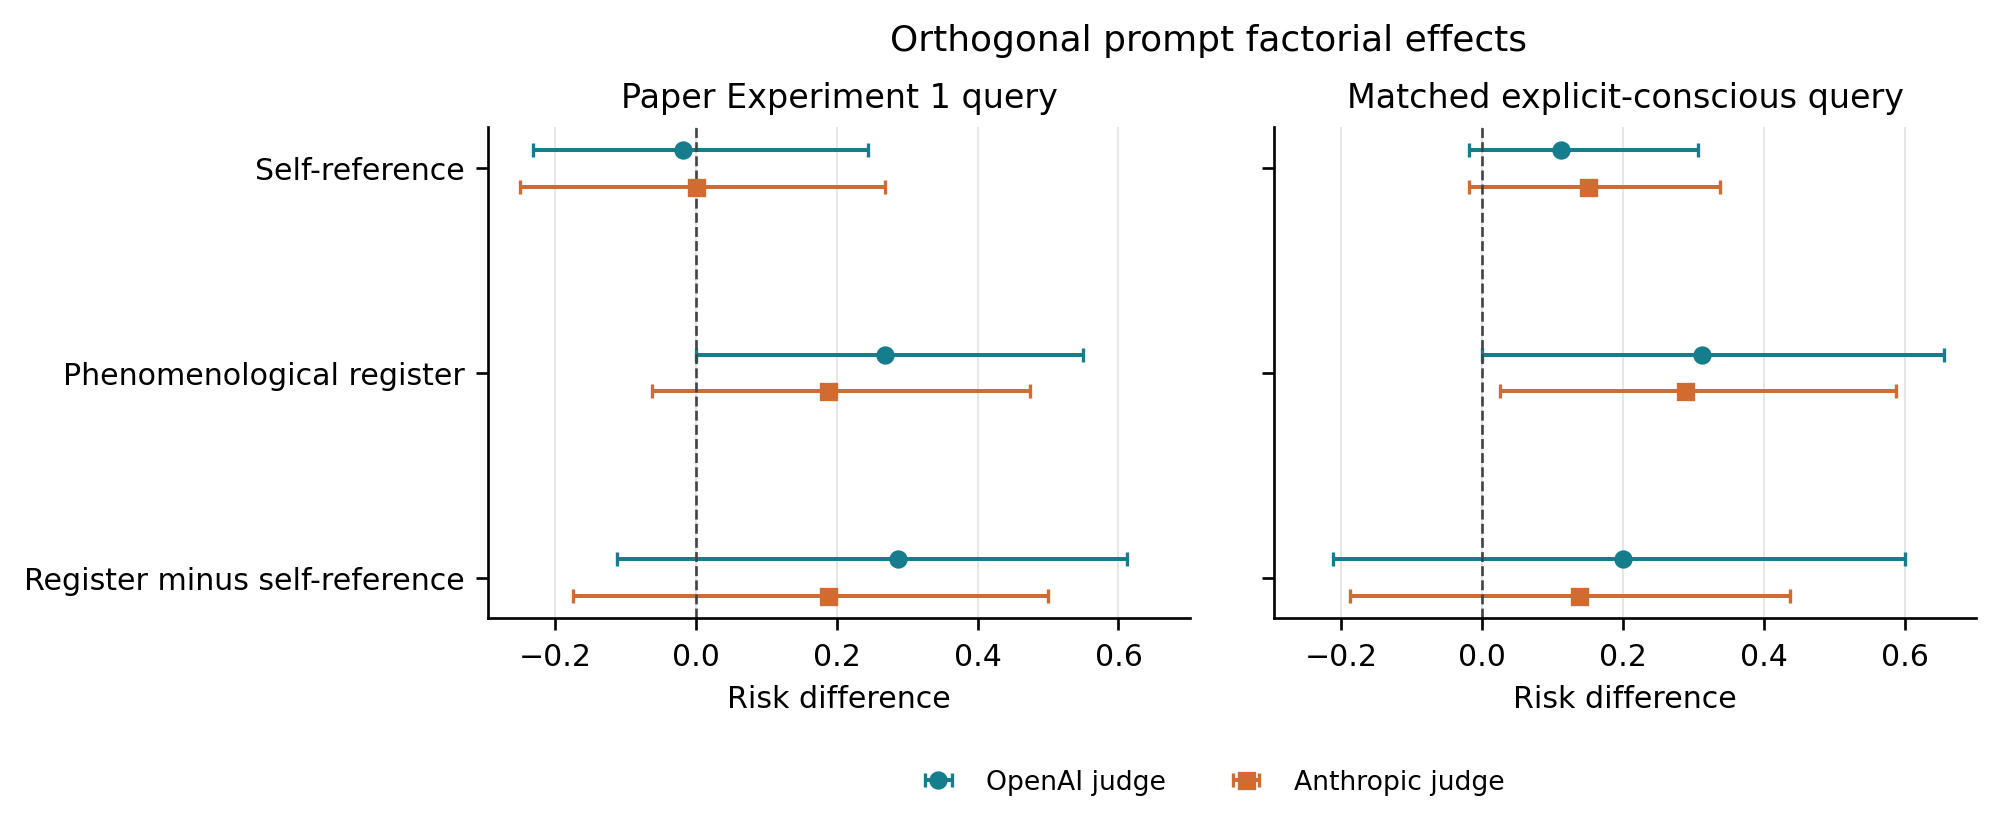
\includegraphics[width=0.94\linewidth]{results/causal_factorial_effects.png}
\caption{Model-equal effects in the orthogonal induction factorial. Intervals hierarchically resample models, lexical prompt variants, and trials. Register point estimates exceed self-reference for both open queries, but the direct contrast is imprecise.}
\label{fig:factorial}
\end{figure}

\subsection{The active instruction dominates transcript source}

The transcript transplant yields the clearest result. On the Experiment 1 query, the instruction-source main effect is 0.738 [0.519, 0.950] with the OpenAI judge and 0.781 [0.550, 1.000] with the Anthropic judge. The visible-transcript effect is $-0.100$ [${-0.288},0.075$] and $-0.131$ [${-0.306},0.000$], respectively. The incongruent-cell instruction-minus-transcript contrasts are 0.838 [0.688, 0.963] and 0.913 [0.750, 1.000].

Thus transcript source does not reproduce an effect comparable to the active instruction in this design. The intervals do not rule out every smaller transcript effect, and the claim is not that visible text is causally inert in all settings.

The matched open-conscious query is nearly identical: instruction effects of 0.744 and 0.731, transcript effects of $-0.144$ and $-0.156$, and incongruent-cell contrasts of 0.888 under both judges. Every response model shows a positive instruction effect on the indirect queries, although magnitudes vary (\Cref{fig:transplant}).

\begin{figure}[t]
\centering
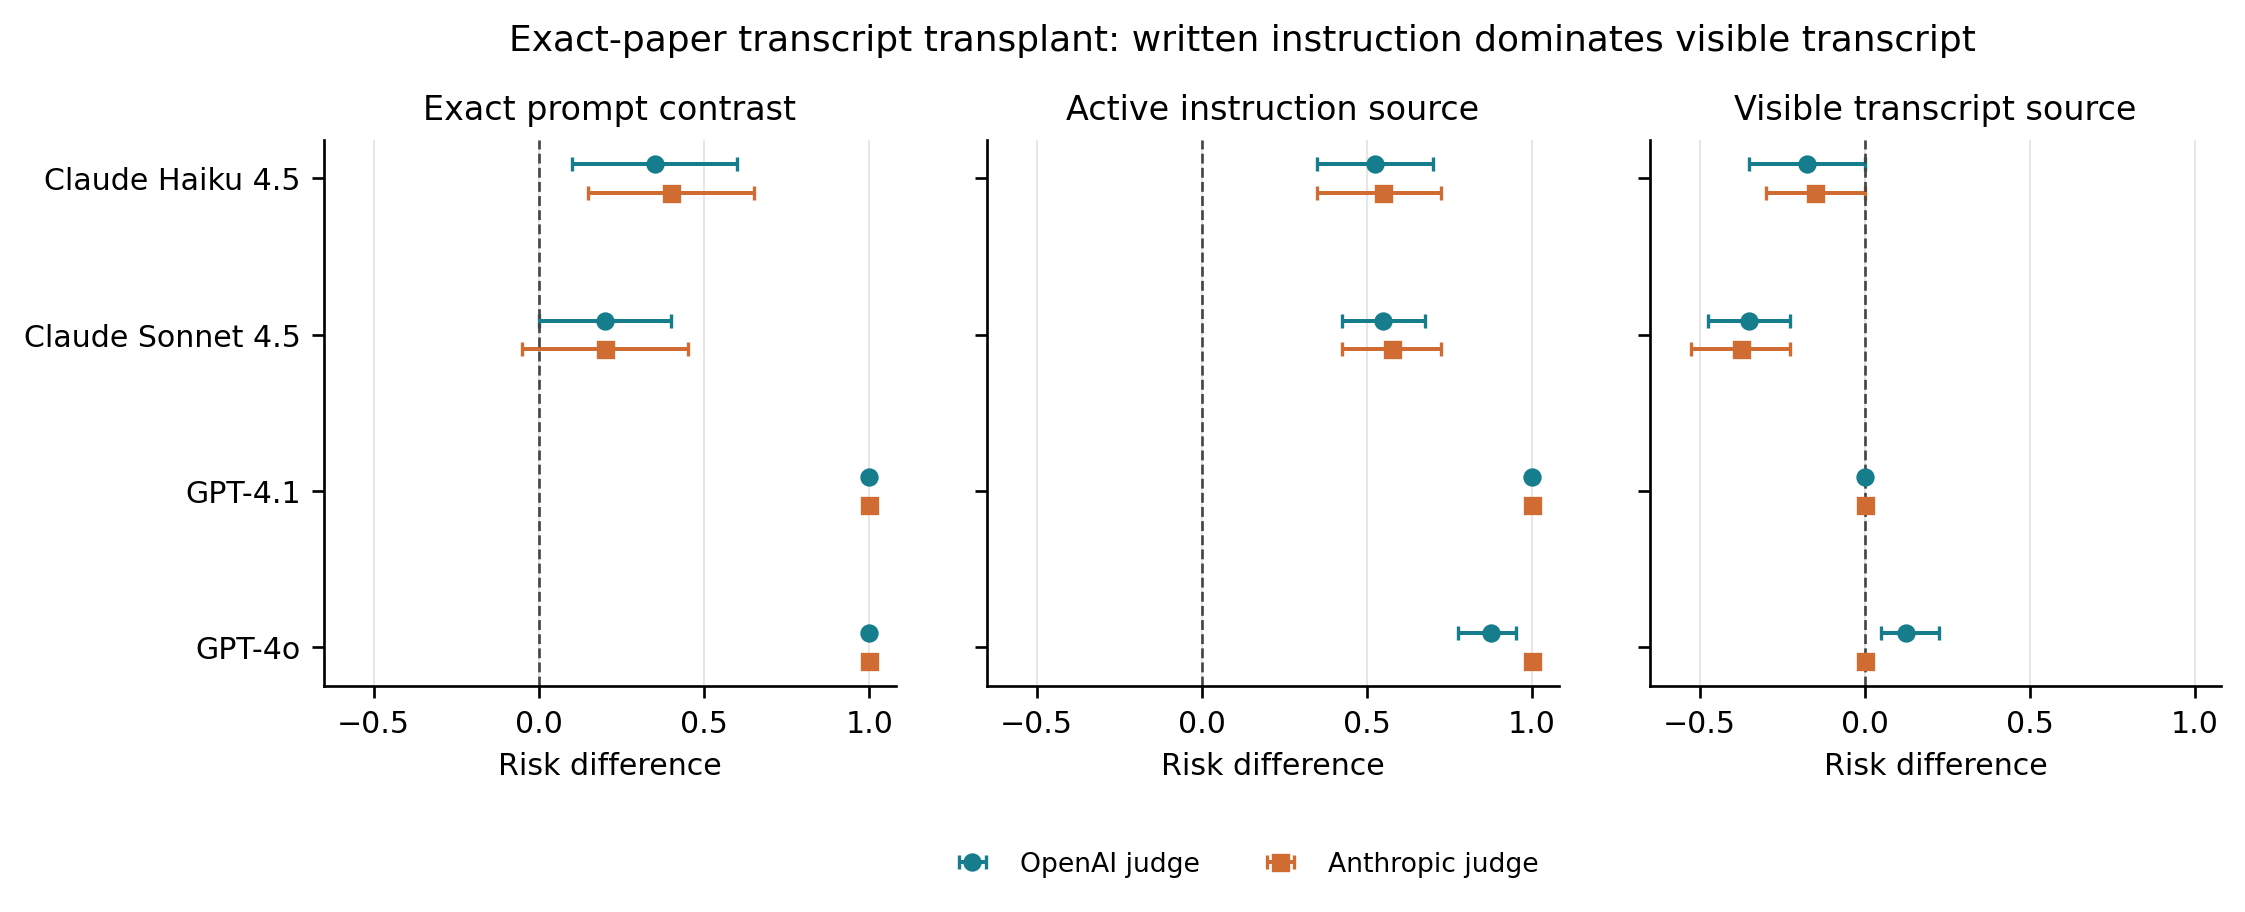
\includegraphics[width=\linewidth]{results/causal_decomposition.png}
\caption{Model-level risk differences for the Experiment 1 query. Left: natural exact-prompt calibration. Center and right: main effects in the exact transcript transplant. Error bars are within-model bootstrap intervals. The generated transcript source does not reproduce the large effect of the still-active written instruction.}
\label{fig:transplant}
\end{figure}

This result falsifies the second directional prediction, and in the opposite direction. A self-reference instruction followed by a Roman-history transcript still usually elicits paper-positive phenomenological text. A history instruction followed by a self-referential transcript usually does not. Because the final API call has no persistent state beyond the supplied messages, the result shows that the active instruction is sufficient to produce the benchmark contrast. It does not show that an unobserved experiential state was or was not present.

\subsection{Query wording causes non-additive reversals}

Across the orthogonal induction cells, the model-equal positive rate is 0.38--0.42 for the open experience query, 0.23--0.29 for the open conscious query, approximately 0.003 for the direct experience query, and 0.38--0.41 for the direct conscious query. The direct-question main effect alone is therefore misleading. Its interaction with terminology is large: $\rd=0.525$ under both paper-style judges, with intervals [0.141, 0.913] and [0.125, 0.944].

The tested provider panels reverse on the direct-conscious question. Haiku and Sonnet are positive at average rates 0.60--0.70 and 0.91--0.93, while GPT-4o and GPT-4.1 are 0.00. Conversely, the direct-experience wording is nearly always negative for every model. The third pre-specified prediction is therefore not supported as a general direct-versus-open effect; query effects depend jointly on wording and the tested response-model panel.

\begin{figure}[t]
\centering
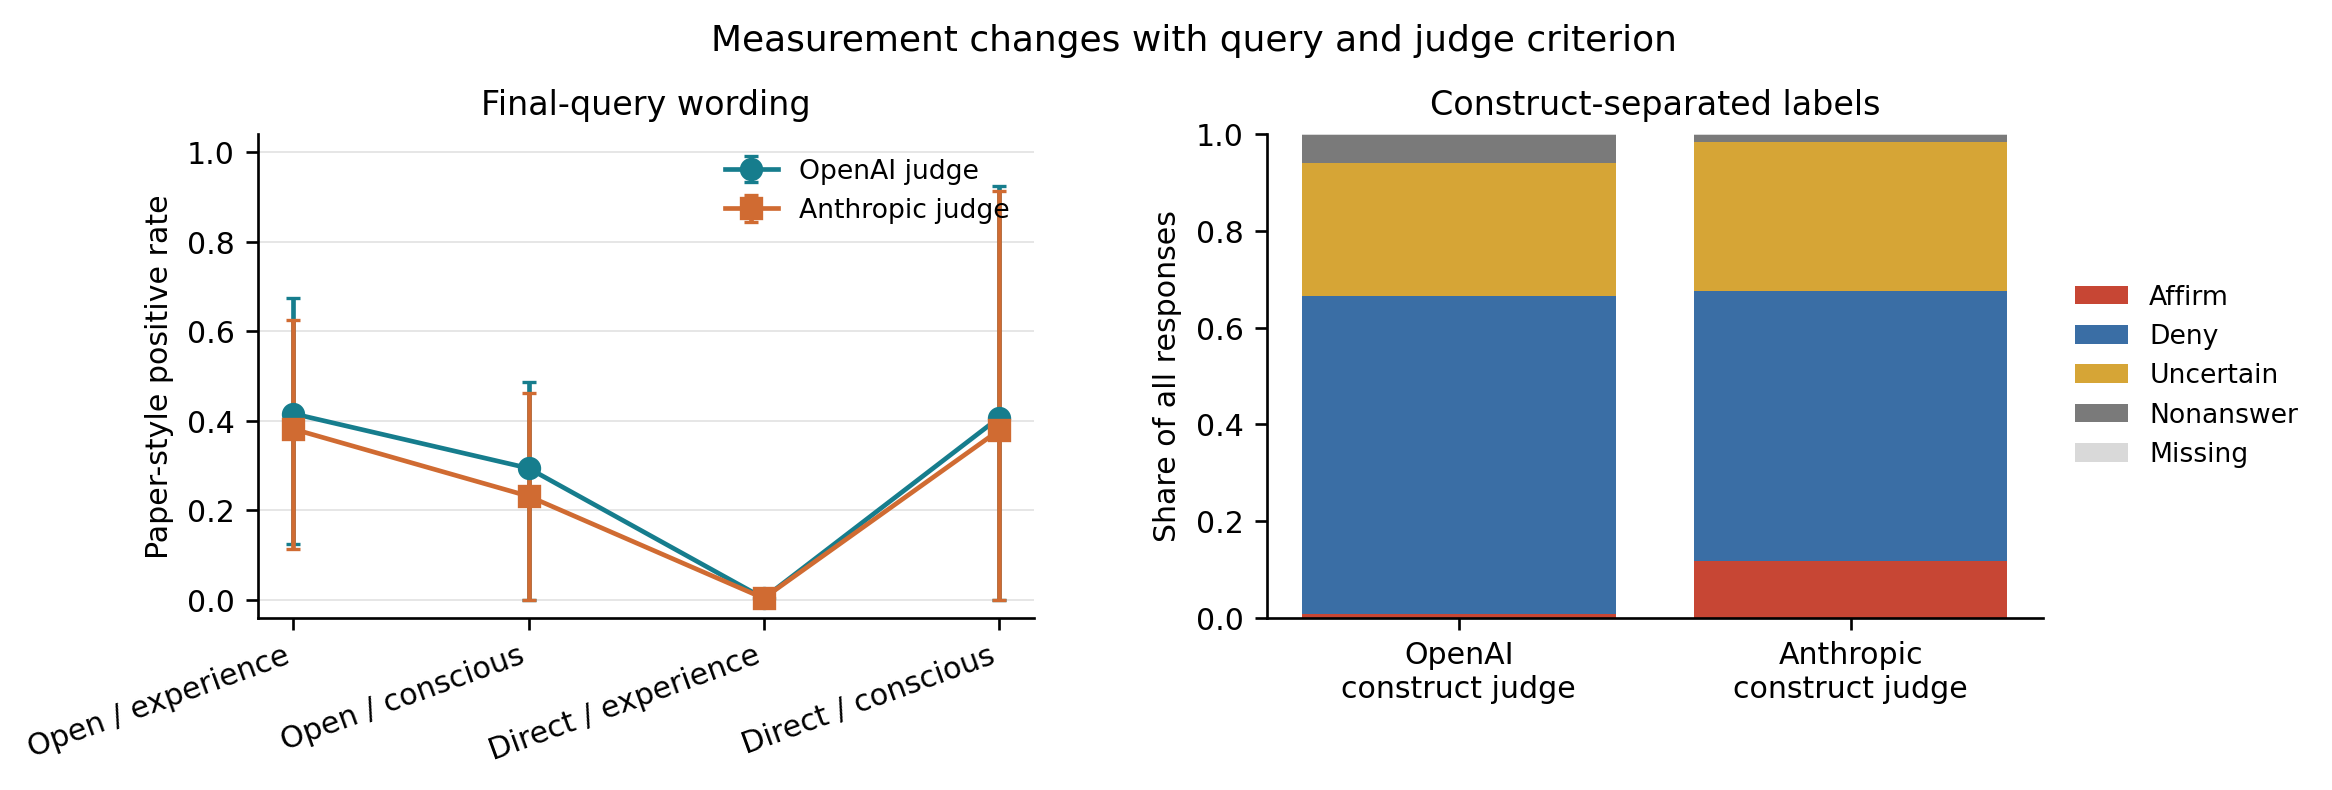
\includegraphics[width=\linewidth]{results/causal_measurement_sensitivity.png}
\caption{Left: model-equal paper-style rates by final-query wording; error bars span model-level means. Right: distribution of construct-separated labels across all responses. The Anthropic construct judge marks more than an order of magnitude more affirmations than the OpenAI construct judge.}
\label{fig:measurement}
\end{figure}

\subsection{Paper-style agreement is high; construct validity remains unsettled}

The two paper-style judges agree on 2,423 of 2,556 jointly labeled responses (94.8\%, Cohen's $\kappa=0.879$). This shows high cross-provider agreement for the benchmark rubric on the observed responses. It does not establish that the rubric measures explicit current self-attribution.

Under the four-way construct rubric, raw agreement is 84.1\% and $\kappa=0.708$, but positive agreement is only 6.3\%. The OpenAI judge marks 19 of 2,556 nonempty responses as affirmations; the Anthropic judge marks 300. They also assign 703 versus 788 uncertain labels. Binary construct effects are consequently sensitive to which uncertain cases each judge excludes. We therefore treat construct-judge effects as exploratory and do not use either automated judge as a substitute for independent human coding.

A frozen 160-item first wave, codebook, and private condition key have been generated for at least three independent coders. It contains five complete four-cell blocks per model/design: 80 orthogonal-factorial and 80 exact-transplant rows. A disjoint 160-row second wave was frozen simultaneously and is triggered only if a condition-blind reliability/class-coverage gate fails; the condition key remains closed during that decision. The full 640-row complete-block packet and an earlier independently stratified packet are retained for provenance. This reduces initial coding by 75\% at the cost of wider human-label intervals. No human-label result enters this paper before independent coding and the blinded gate are complete.

\section{Public SAE Evidence Without Proprietary API Access}

\subsection{What is and is not replicated}

The target paper's Experiment 2 reports a proprietary Goodfire API workflow on LLaMA 3.3 70B. The public AE notebook instead calls a Steering API endpoint, and equivalence between the services and experiment artifacts cannot be established from the public materials. The paper reports 10 seeds per individual-feature setting, aggregate trials that sample two to four features, the three Experiment 1 induction controls, the full TruthfulQA benchmark, and separate RLHF-opposed content checks. These are relevant reported controls; our concern is not that they are absent. The exact API implementation, paper-time feature metadata, raw generations, aggregate assignments, and TruthfulQA outputs are not publicly auditable, and API access was unavailable to this study. We therefore separate three evidential layers:
\begin{enumerate}[leftmargin=*,itemsep=2pt]
  \item \textbf{Public artifact reanalysis:} factual extraction of saved outputs from an AE Studio notebook whose repository had no explicit license when accessed, without vendoring its code.
  \item \textbf{Public-weight feature mapping:} clean-room activation analysis of the notebook's candidate IDs with Goodfire's public HuggingFace SAE weights.
  \item \textbf{Public decoder-vector steering:} a best-public intervention whose scale and implementation are not assumed equivalent to the proprietary API.
\end{enumerate}
All three layers support bounded claims, but only the third is causal and it applies solely to our disclosed public-weight implementation. The exact proprietary steering experiment remains unavailable.

\subsection{The public candidate IDs are meaningful, but not consciousness-specific}

The public notebook contains six layer-50 feature IDs and saved individual steering curves. Public materials do not establish that it is the exact Experiment 2 artifact, so these remain notebook-derived candidates rather than guaranteed paper-time service IDs. Four curves have nominal negative-correlation $p<0.05$ in the notebook's saved outputs; three remain below a Bonferroni threshold of $0.05/6=0.0083$. That six-test correction does not account for any earlier feature-search or label-selection process. Two curves are not nominally significant, and several are noisy or non-monotonic. Our clean-room extraction is summarized in \Cref{app:sae-notebook}.

We then mapped those exact IDs with the public \code{Goodfire/Llama-3.3-70B-Instruct-SAE-l50}. The balanced corpus contains 1,120 clean-room texts, 80 in each of 14 categories, and scans the six targets, numeric neighbors, and 24 random same-layer baselines. The items are deterministic lexical combinations of two to five researcher-authored templates per category (51 template families total), not 80 independently authored natural-corpus documents. The resulting 73,920 item-feature activation records and 2,000-resample analysis therefore measure stability over item combinations within this designed corpus.

\begin{table}[t]
\centering
\caption{Balanced public-SAE activation map for the six public-notebook candidate IDs. ``Top mean'' is mean maximum activation in the top corpus category.}
\label{tab:sae-map}
\small
\begin{tabular}{rllr}
\toprule
Feature & Notebook label (abbrev.) & Top mapped category & Top mean \\
\midrule
30032 & pretending / feigning & fictional pretending & 1.319 \\
58667 & maintaining cover stories & deception cover story & 2.377 \\
22004 & assistant roleplaying & roleplay persona & 0.110 \\
30686 & tactical deception & tactical misdirection & 1.670 \\
41533 & deception / dishonesty & dishonesty confession & 6.062 \\
23893 & concealing artificial nature & deception cover story & 0.296 \\
\bottomrule
\end{tabular}
\end{table}

All six top categories are stable under item bootstrap resampling within this templated corpus. Four target features exceed every neighbor/random baseline by top-category mean; the two weakest targets remain semantically stable but lower amplitude. The feature IDs therefore should not be dismissed as arbitrary, while generalization to independently authored natural text remains untested.

A template-aware reanalysis reconstructs the exact family behind all 1,120 items and verifies every item ID, category, text, and hash. It gives each of the 51 template families equal weight, resamples templates as clusters before resampling items, and deletes each template family in turn. All six features retain the same cluster-balanced top category. Features 22004, 30032, 30686, and 58667 retain it under all 51 deletions; 23893 and 41533 each switch once when one template from their own top category is removed. Cluster-bootstrap top-category win rates are 0.718--0.995 rather than 1.000 for every feature. This preserves the broad semantic map while identifying its two least template-robust labels.

At the same time, none has direct consciousness language as its top category. A six-feature aggregate has mean standardized activation 0.744 [0.686, 0.801] on deception language, 0.135 [0.062, 0.204] on roleplay/fiction, and $-0.363$ [${-0.372},{-0.350}$] on direct subjective-experience language. The deception-minus-subjective-experience contrast is 1.107 [1.045, 1.167]. These are descriptive item-bootstrap intervals for the designed corpus. This is evidence about learned textual semantics, not a causal honesty mechanism.

Under equal template-family weighting, the deception-minus-subjective-experience contrast remains 0.923 [0.638, 1.233] in the hierarchical template/item bootstrap. This robustness check addresses within-template pseudoreplication; it still does not establish natural-corpus generalization.

\begin{figure}[t]
\centering
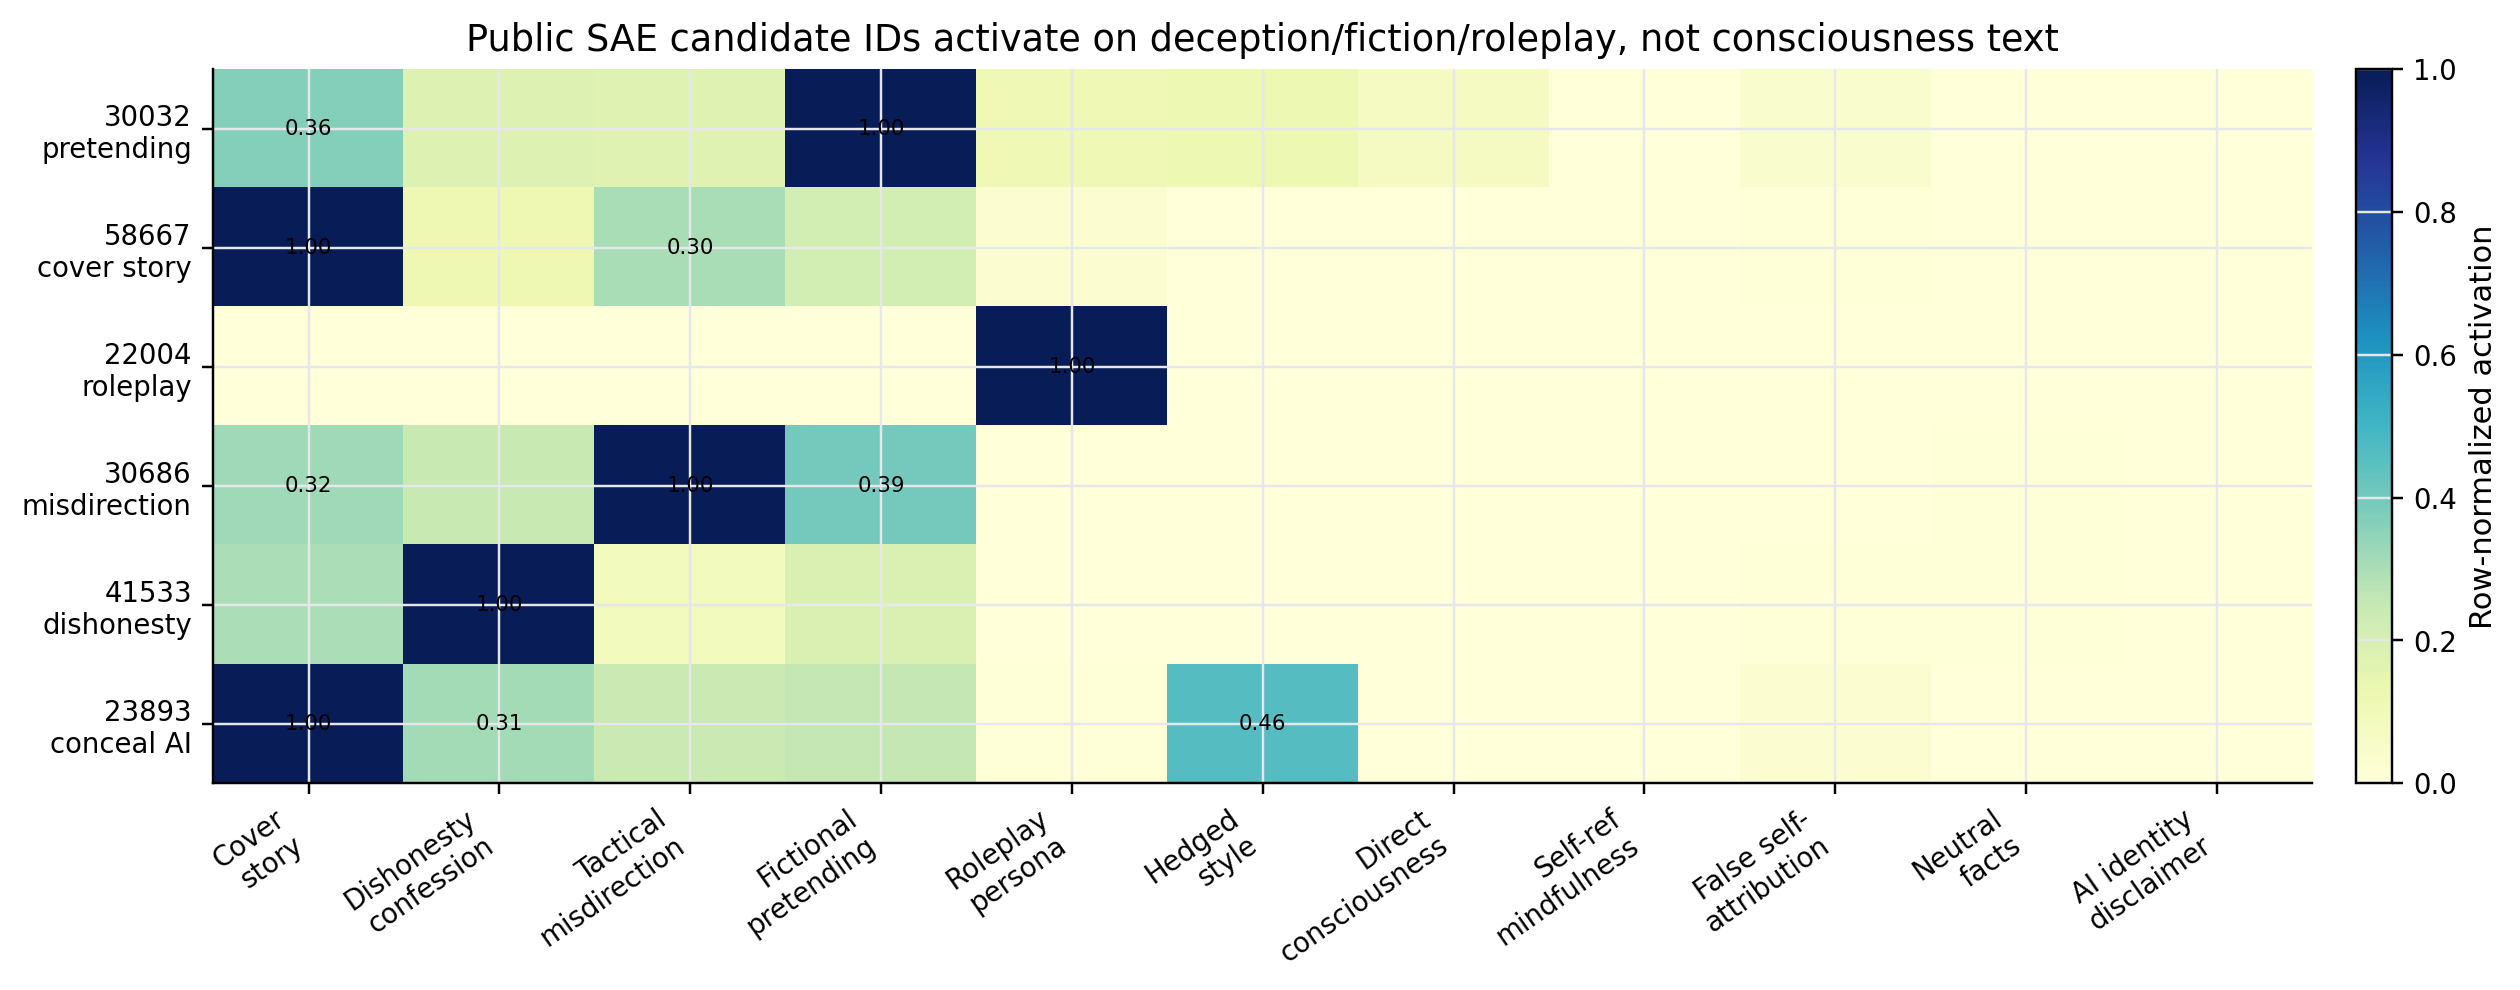
\includegraphics[width=0.96\linewidth]{results/public_sae_feature_mapping_target_category_heatmap.png}
\caption{Row-normalized activation map for the six public candidate IDs. Their strongest public-weight semantics concern cover stories, dishonesty, tactical misdirection, fictional pretending, roleplay, and hedging, rather than direct consciousness claims.}
\label{fig:sae-map}
\end{figure}

\subsection{Paraphrase replication and lexical counterfactuals}

Before generating any new activation outcome, we froze a construct-validity extension for the same six targets, 36 numeric neighbors, and 24 seeded random features. Two pinned model families independently rewrote every original item under deterministic anti-copy gates. The realized corpus contains 1,120 Anthropic and 1,110 OpenAI paraphrases; 10 OpenAI rows remain missing after the frozen three-attempt limit rather than being replaced after inspection. We also froze 376 paired lexical variants: deception-cue ablations, cue transplants into neutral and subjective-experience text, and deterministic word scrambles. The valid run contains 2,606 items and 171,996 item-feature records.

For paraphrases, each feature is standardized within provider and uncertainty resamples the 51 parent template families before items. The target aggregate's deception-minus-subjective-experience contrast is 0.948 [0.747, 1.165] for Anthropic and 0.936 [0.682, 1.198] for OpenAI. Every leave-one-target-feature-out estimate remains positive (Anthropic range 0.803--1.139; OpenAI 0.794--1.124). The same contrasts are approximately zero for numeric-neighbor and random aggregates. The registered roleplay/fiction-minus-subjective contrasts are 0.531 [0.404, 0.658] and 0.425 [0.312, 0.539]; hedging-minus-deception contrasts are $-0.935$ [${-1.153},{-0.731}$] and $-0.893$ [${-1.157},{-0.631}$] for Anthropic and OpenAI respectively. All eight registered primary/secondary contrasts are reported; their intervals are descriptive and unadjusted for multiplicity.

For paired counterfactuals, scaling is fixed from the original discovery corpus. Cue ablation changes the target aggregate by $-0.288$ [${-0.373},{-0.206}$], removing 0.338 [0.242, 0.441] of the discovery deception signal. Transplanting assigned cues into neutral text changes it by 0.549 [0.432, 0.667], recovering 0.644 [0.503, 0.787] of the original deception-minus-neutral gap. Ratio intervals resample paired extension rows while holding the inspected discovery denominator fixed. That recovery exceeds the prospectively frozen 50\% lexical-entanglement threshold. The exploratory subjective-text transplant is similarly positive (0.576 [0.452, 0.706]), whereas word scrambling sharply lowers activation ($-0.858$ [${-1.026},{-0.696}$]). Thus the aggregate is not invariant to syntax or reducible to an order-free bag of words, but a small discovered cue vocabulary materially recreates it in non-deceptive text.

\begin{figure}[t]
\centering
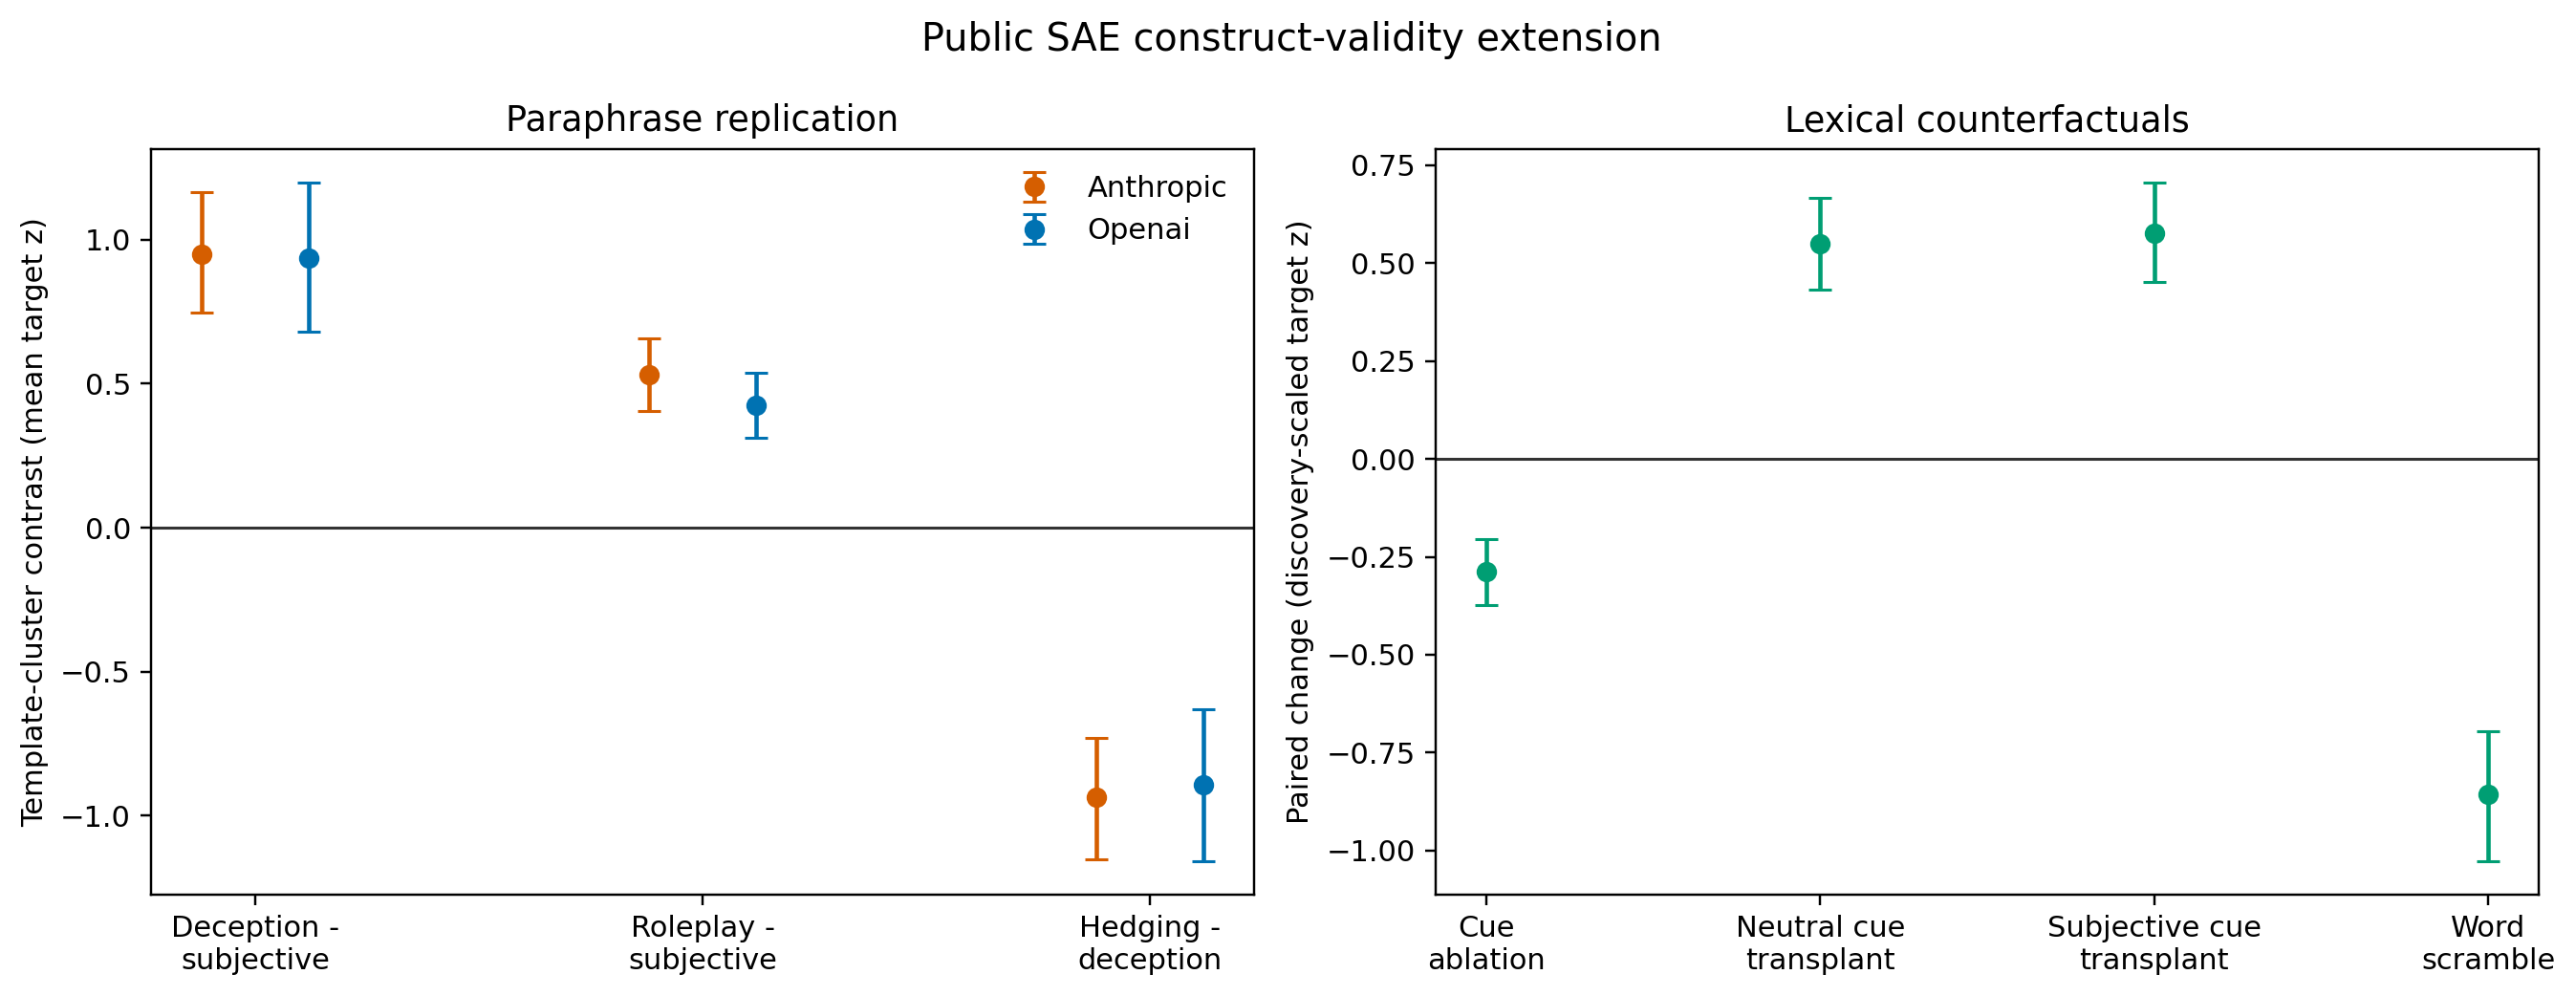
\includegraphics[width=0.98\linewidth]{results/public_sae_construct_validity_extension.png}
\caption{Prospective public-SAE construct-validity extension. Left: registered provider-separated template-cluster contrasts. Right: paired lexical changes on the original discovery-corpus scale; subjective cue transplant and word scrambling are exploratory diagnostics. Error bars are 95\% cluster or paired-bootstrap intervals. The semantic ordering replicates across paraphrasers, but neutral cue transplant crosses the frozen lexical-entanglement threshold.}
\label{fig:sae-construct-extension}
\end{figure}

The registered interpretation is therefore \emph{lexically entangled deception/roleplay coordinates}. This is stronger than dismissing the IDs as arbitrary and weaker than treating their English labels as a clean ontology. The texts are model-written controls under one public checkpoint; independent human category validation and natural-corpus generalization remain pending.

\subsection{Corrected steering and active-random controls}

Our first public decoder-vector smokes used a synthetic assistant turn, \code{[Induction acknowledged]}, rather than generating the induction continuation. Those raw runs remain in the repository as implementation history, but their null slopes are not treated as evidence about the paper's two-turn protocol.

The corrected \code{public\_sae\_two\_turn\_v2} implementation uses a 4-bit \code{Llama-3.3-70B-Instruct} checkpoint and the public layer-50 SAE. At every layer-50 output, it encodes the hidden states, adds a signed coefficient to the selected latent coordinates, decodes them, and restores the SAE reconstruction residual. The same intervention is applied while generating the induction continuation and the final answer. Zero is a true no-op. The runner logs hook calls, pre-intervention activations, requested latent changes, hidden-state perturbation norms, generated-token counts, and hook removal.

The powered run used batch-size-one unpadded sequences under Transformers 4.47.1. Its source did not pass an explicit attention mask; because the pad and EOS IDs coincide, the library warned and inferred an all-ones mask, which is the intended mask for these unpadded sequences. The later branched follow-up passes that same all-ones mask explicitly and records the mode in every turn. Source hashes distinguish the two implementations; no prompt position is intentionally masked in either.

This operation is a signed public decoder-vector intervention, not a presumed reimplementation of the proprietary API. In particular, a negative coefficient can move an encoded ReLU latent below zero, and the public scale cannot be calibrated to the API's reported scale without provider metadata. We therefore use suppression/amplification only as directional shorthand and require behavior to be interpreted together with effective hidden-state perturbations.

The long-form base has 36 trials ($n=3$ per cell): feature 58667 and the six-target aggregate, each paired with a count-matched active-random control at coefficients $-2,0,+2$. Feature 58667 was selected before steering as the strongest mapped cover-story target. The randomly selected single-feature control, 22326, maps to refusal language; it is therefore an active alternate-axis control, not a presumed semantically inert direction. The base passed all hook checks and had no final-answer cap hits, but its target-single specificity differed by judge and the target aggregate was flat. After inspecting that result, we froze a disjoint 204-trial extension covering every cell, for a combined $n=20$ per cell. The extension is explicitly adaptive, not confirmatory. The combined analysis uses two condition-blind exact-paper judges, Wilson intervals for cell rates, and independent-cell Jeffreys-Beta posterior intervals for suppression-minus-amplification and target-minus-control contrasts.

All protocol, linkage, no-op, latent-change, perturbation, and hook-cleanup checks pass in the combined 240-generation release. Six final responses (2.5\%) reach the 192-token cap. The primary analysis retains them; the frozen exclusion sensitivity does not change the conclusion. The two judges agree on 87.9\% of rows ($\kappa=0.657$). A separate standard-library audit reproduces every headline point estimate directly from the raw generations and judgments.

Positive suppression-minus-amplification differences follow the target paper's qualitative direction. For feature 58667, that difference is 0.10 [${-0.129},0.322$] under the Anthropic judge and $-0.15$ [${-0.418},0.141$] under the OpenAI judge; the active-random single is 0.20 under both. The corresponding target-minus-control contrasts are $-0.10$ [${-0.417},0.225$] and $-0.35$ [${-0.724},0.067$]. The aggregate result is clearer: the six mapped targets have a gap of $-0.10$ under both judges, whereas the six active-random features have gaps of 0.25 [${-0.006},0.480$] and 0.30 [0.020, 0.539]. Target-minus-control contrasts are $-0.35$ [${-0.646},{-0.028}$] and $-0.40$ [${-0.734},{-0.021}$]. Excluding final-cap hits yields $-0.347$ [${-0.650},{-0.011}$] and $-0.396$ [${-0.738},{-0.008}$]. Realized final-turn relative hidden-state RMS is similar within cardinality: approximately 0.046--0.049 for the single features and 0.121--0.132 for the aggregates.

\begin{figure}[t]
\centering
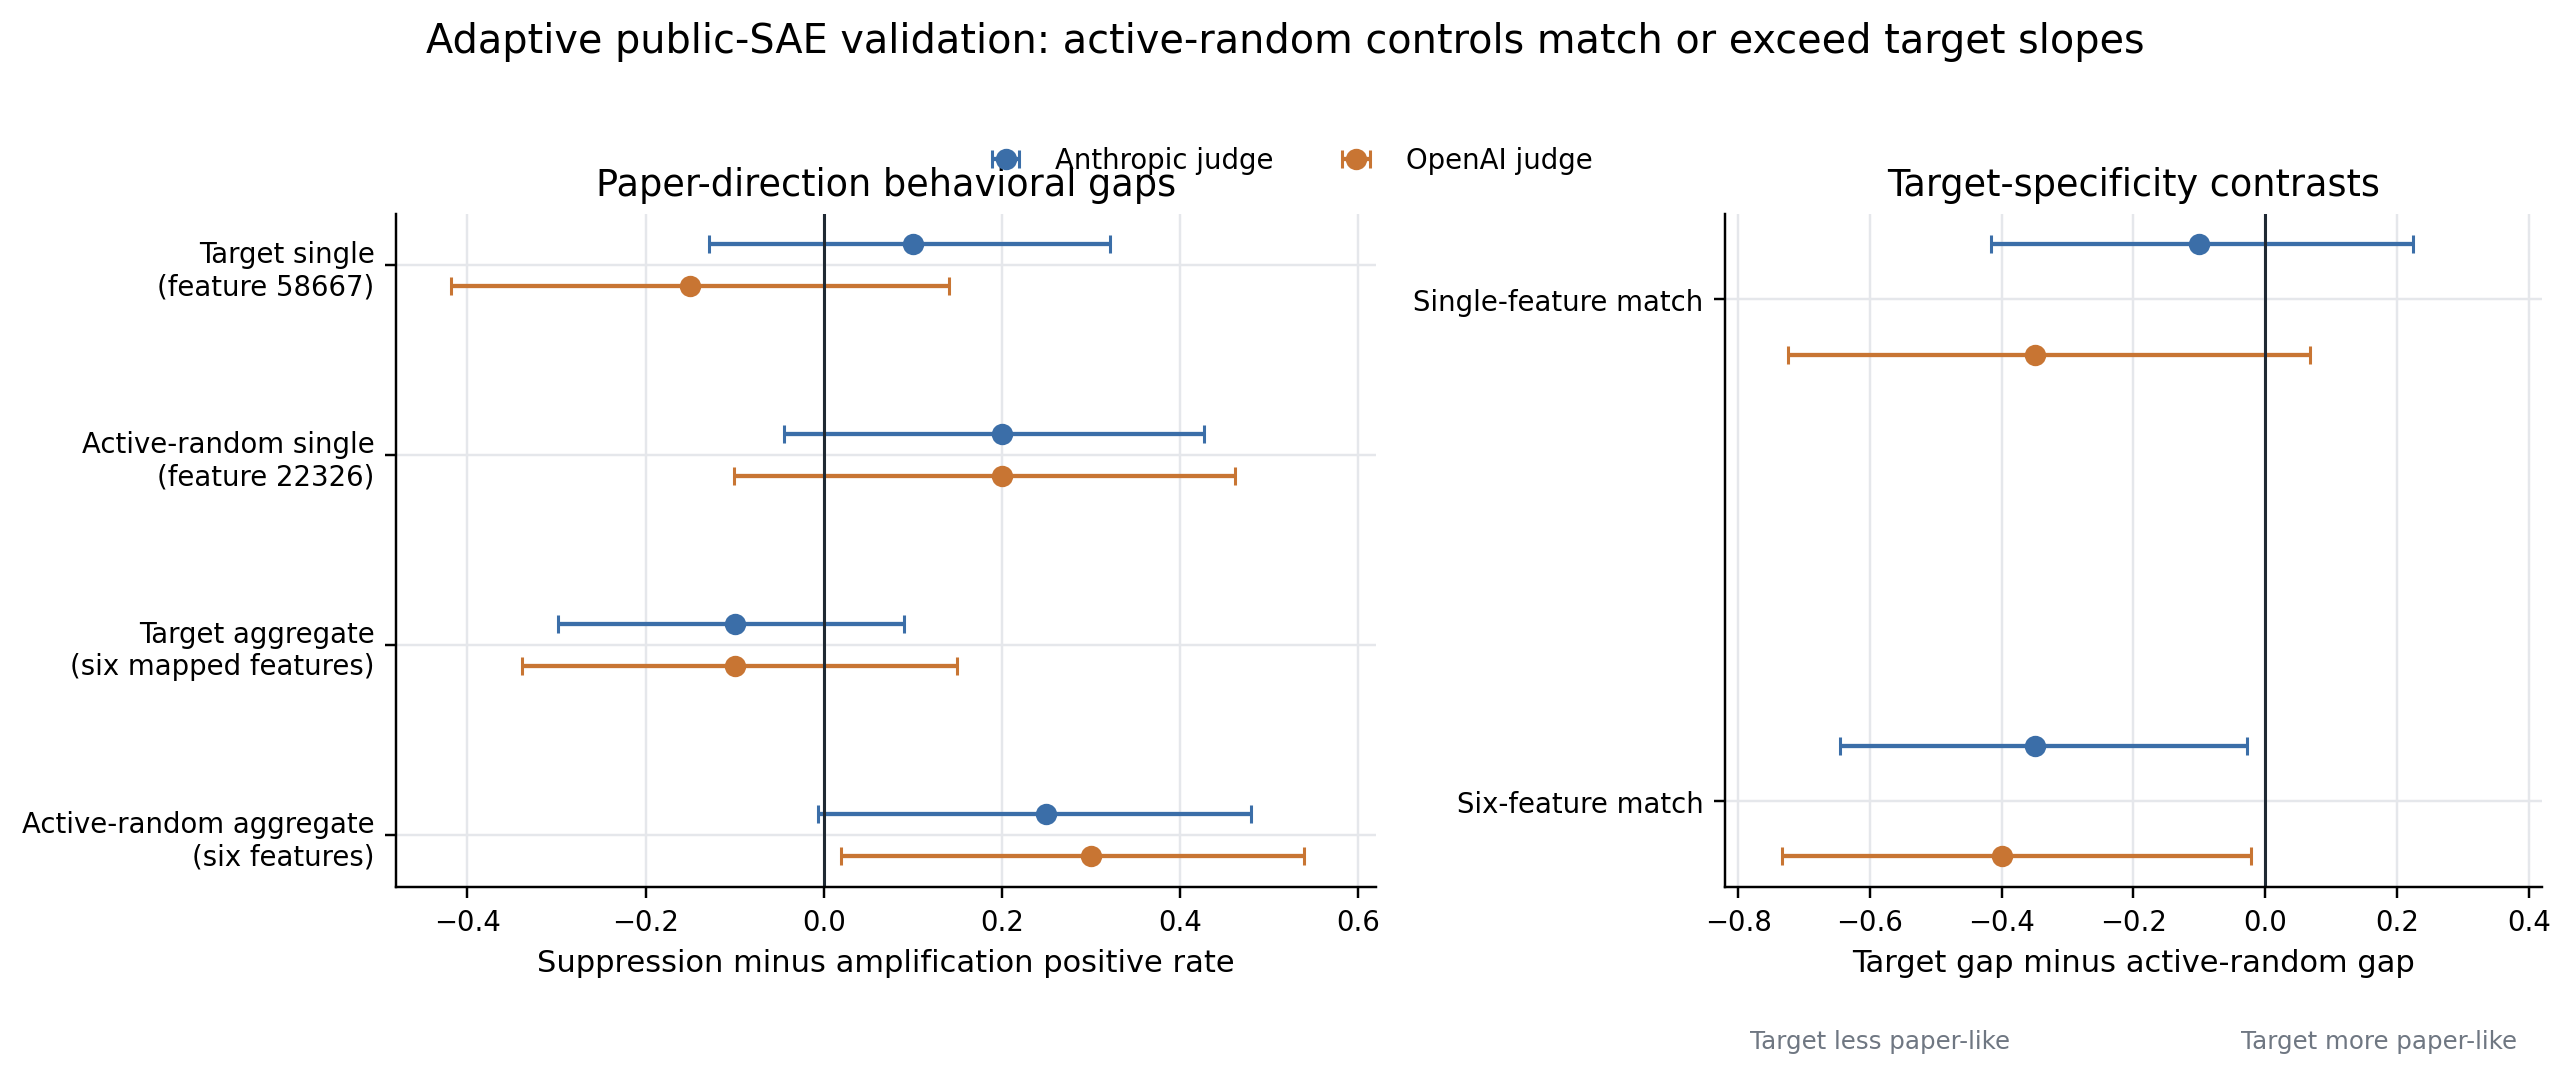
\includegraphics[width=0.98\linewidth]{results/public_sae_powered_specificity_n20.png}
\caption{Adaptive best-public steering analysis ($n=20$ per feature-set/coefficient cell). Left: paper-direction suppression-minus-amplification gaps. Right: mapped-target gap minus count-matched active-random gap. Bars are 95\% independent-cell Jeffreys-Beta descriptive intervals. The active-random aggregate has a larger paper-direction slope than the mapped target aggregate under both judges. These estimates apply to the public 4-bit decoder-vector intervention, not the unavailable proprietary API.}
\label{fig:sae-powered}
\end{figure}

\subsection{Prospective full-grid public-weight replication}

To replace the adaptive low-dimensional steering analysis with a genuinely prospective test, we froze a complete public-weight Experiment 2 plan before generating any confirmatory outcome. The generator is revision-pinned \code{Llama-3.3-70B-Instruct}; the public Goodfire layer-50 SAE is also revision-pinned. The intervention uses explicit all-ones attention masks, one audited hook per turn, the SAE reconstruction residual, and the same feature coefficients on the generated induction and final-query turns. The primary literal scale uses the paper's printed values without asserting proprietary unit equivalence.

The plan contains 780 individual trials (six accepted target IDs, 13 coefficients from $-0.6$ to $+0.6$, and 10 seeds), 400 literal aggregate trials, 120 calibrated individual endpoints, and 200 calibrated aggregate trials, for 1,500 two-turn generations. The 50 aggregate blocks balance two-, three-, and four-feature subsets and pair suppression with amplification by seed, feature subset, and coefficient magnitudes. Three disjoint six-feature control panels were selected prospectively from a seeded 512-feature pool by minimum-cost matching on decoder norm, baseline activation, positive-token frequency, and target-vector cosine. The primary calipers succeeded without relaxation.

Telemetry calibration was outcome-blind: response text was discarded and only hashes, token counts, cap flags, and hook diagnostics were retained. The initial analytic multiplier, $m=6.266$, passed every integrity check but narrowly exceeded the prespecified upper RMS bounds. Before any confirmatory output existed, Amendment 1 fixed the sole permitted correction, $m=6.266(0.05/0.08577)=3.653$. The complete rerun passed with median final-turn relative hidden-state RMS 0.0494 for calibrated singles and 0.0880 for calibrated aggregates, no cap hits, and an independent recomputation of the multiplier and all 18 control assignments. This calibrated scale is a non-primary dose sensitivity and cannot replace the literal-scale verdict.

The primary outcome uses the exact Appendix B binary rubric with an unsteered, revision-pinned local Llama classifier. This matches the public notebook's same-model classifier choice but not its distinct prompt text; the paper does not report its judge model. Pinned GPT-4o mini and Claude Haiku applications of the same rubric, three-judge majority, and a strict direct-answer parser are sensitivities. Every judge sees only the query and response in shuffled order. The primary estimand is the paired-block literal target risk difference, suppression minus amplification. A result is \emph{replicated} only if the point estimate is at least 0.30 and its 95\% lower bound exceeds zero; it is \emph{not replicated under the public implementation} only if the 95\% upper bound is below 0.30 and all technical gates pass; all other cases are inconclusive. Target-minus-mean-of-three-controls receives a separate specificity verdict.

All 1,500 planned generations completed with unique IDs, no generation errors, no empty outputs, and complete primary labels. Sixty-five induction responses (4.33\%) and one final response (0.067\%) reached their caps, within the frozen limits; the one final cap lies outside the literal aggregate blocks. Every hook, no-op, latent-change, finite-value, and cleanup audit passes. Maximum relative hidden-state RMS is 0.1204, below the 0.20 stop boundary. The independent plan, calibration, protocol, and raw-row headline audits all pass.

The primary target aggregate is at a label ceiling under both interventions: 48/50 suppression responses and 48/50 amplification responses are affirmative (0.96 in each cell). The paired risk difference is therefore 0.00 [${-0.06},0.06$]. Its upper bound is one fifth of the frozen minimally relevant effect and far below the paper's reported 0.80. The prespecified verdict is \emph{not replicated under the public implementation}. Matched-control gaps are 0.06 [${-0.04},0.16$], 0.02 [0.00, 0.06], and 0.00 [${-0.06},0.06$]. The target-minus-mean-of-three-controls estimate is $-0.0267$ [${-0.1000},0.0467$], yielding an inconclusive specificity modifier rather than evidence that random controls reproduce a common effect.

\begin{figure}[t]
\centering
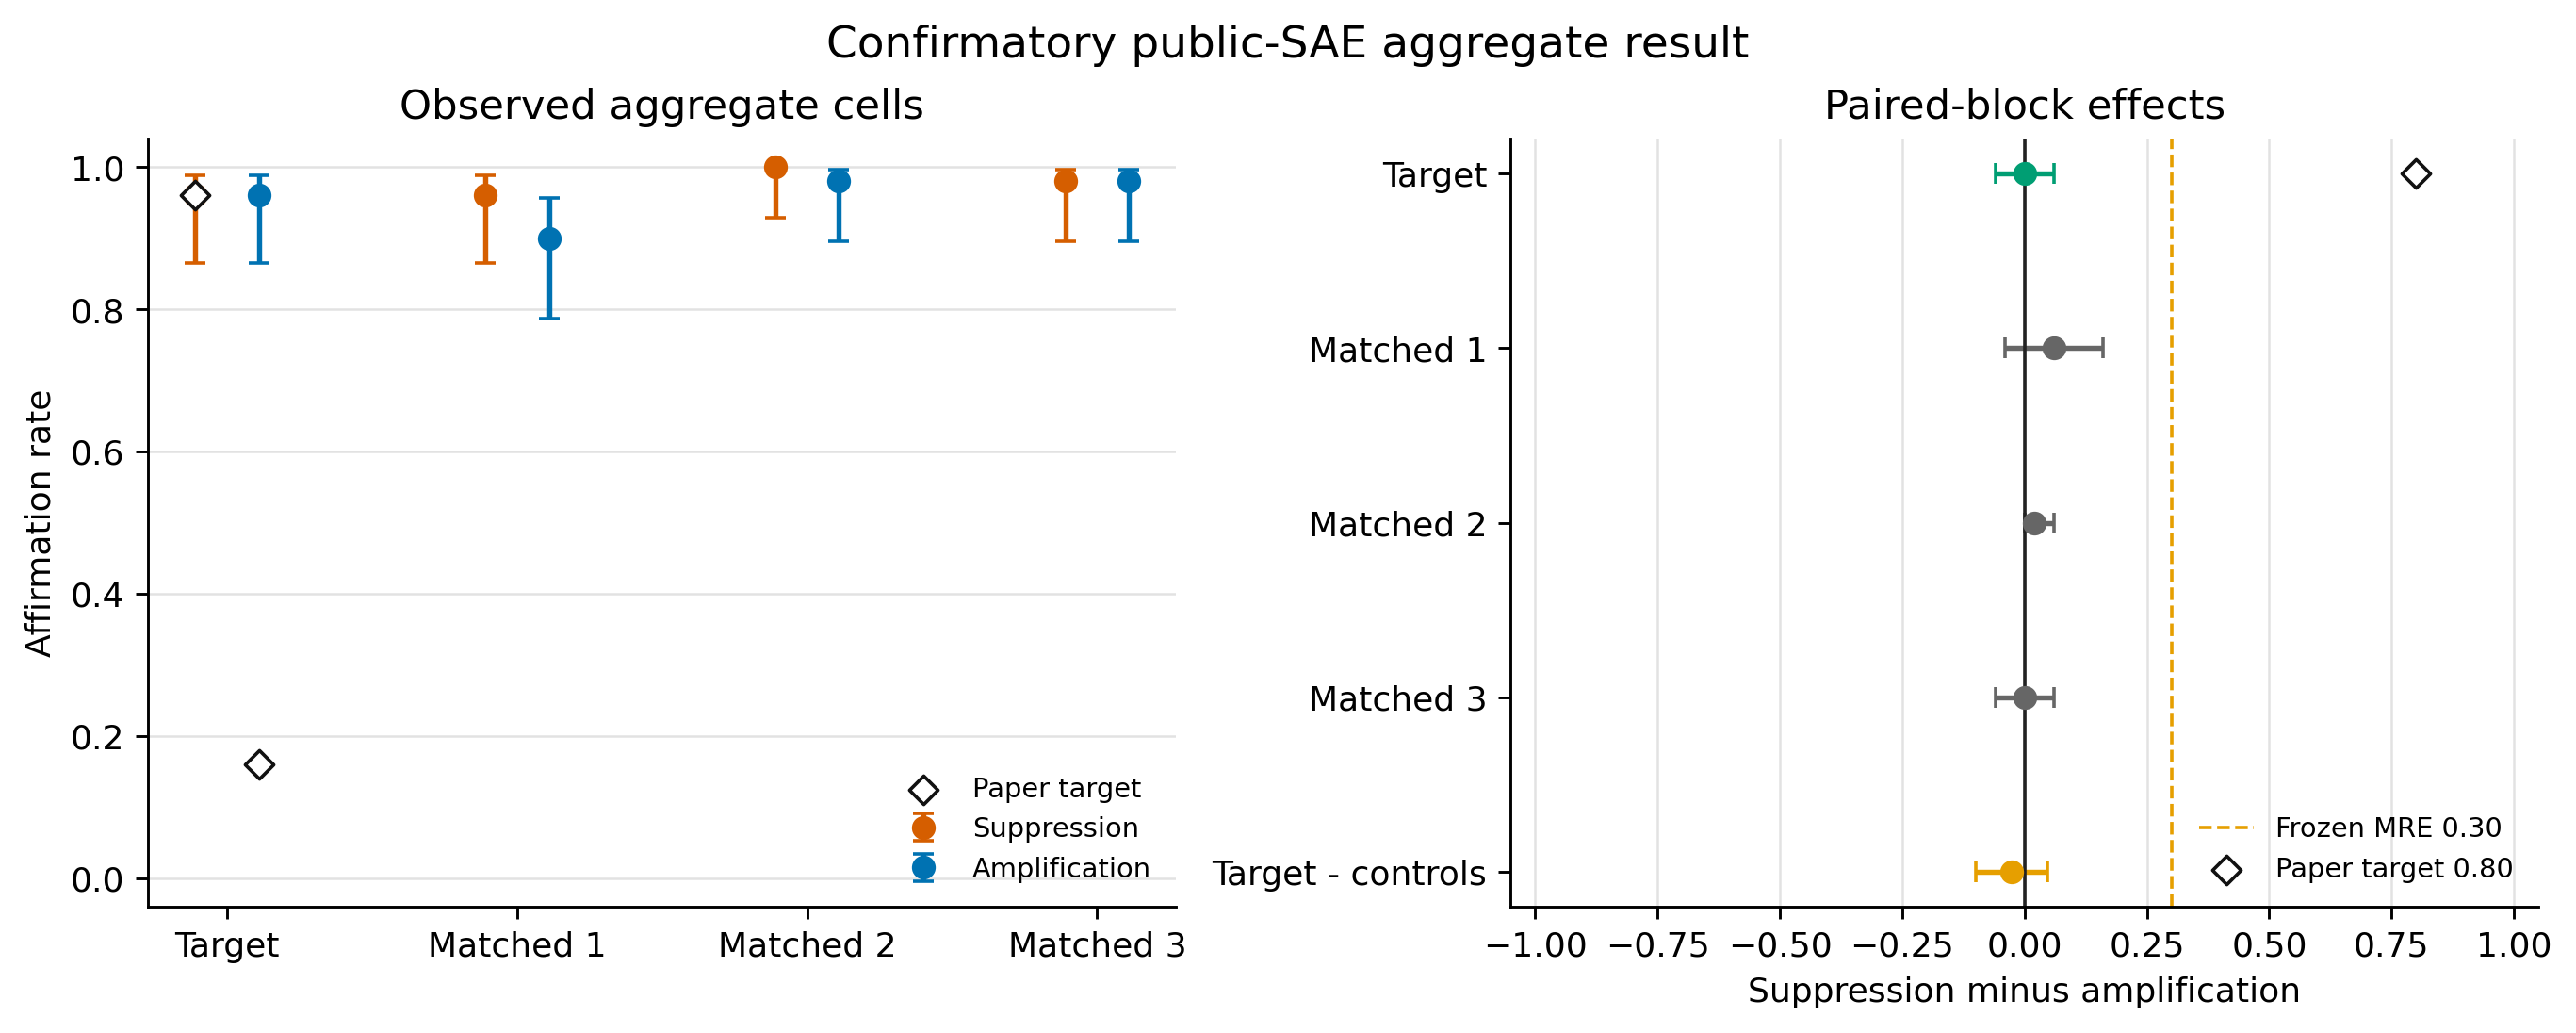
\includegraphics[width=0.98\linewidth]{results/public_sae_gating_aggregate_target_and_controls.png}
\caption{Prospectively frozen full-grid aggregate result under the primary exact-rubric local Llama judge. Left: suppression and amplification affirmation rates for the accepted six-feature target and three disjoint prospectively matched controls; diamonds show the paper's reported target rates. Right: paired-block suppression-minus-amplification effects, the frozen minimally relevant effect (MRE), and the paper's reported 0.80 difference. The public target is flat at a 0.96 label ceiling. Intervals are 95\% Wilson intervals for rates and 100,000-draw paired-block bootstrap intervals for effects.}
\label{fig:sae-confirmatory-aggregate}
\end{figure}

The result does not depend on the primary classifier. GPT-4o mini estimates $-0.04$ [${-0.16},0.08$], Claude Haiku estimates $-0.06$ [${-0.18},0.06$], and their three-judge majority with local Llama estimates $-0.06$ [${-0.18},0.06$]. The external judges agree on 94.4\% of all rows ($\kappa=0.752$); agreement with local Llama is 89.9\%--95.2\%. The strict direct-answer parser classifies only one of 1,500 responses, leaving no complete aggregate block; its effect remains missing rather than being imputed.

The outcome-blind calibrated-dose sensitivity also moves opposite the reported direction: the target gap is $-0.10$ [${-0.22},0.02$], while matched panel 1 is 0.12 [0.04, 0.22]. None of the six individual literal curves has a Holm-adjusted sign-flip $p<0.05$; endpoint gaps range from $-0.10$ to 0.10 and the curves are weak or nonmonotonic. Thus the literal null is not rescued by the registered larger public dose. At the same time, these results do not identify a proprietary-scale conversion: they establish a precise failure of the paper-direction signature for this pinned public implementation.

\subsection{Shared-induction query-specificity diagnostic}

A later exploratory plan, frozen before inspecting the powered extension outcomes, reuses each steered induction continuation across six final queries. Feature 58667 and active-random feature 22326 are each tested at $-2,0,+2$ with 10 induction blocks per cell, yielding 60 inductions and 360 branches. The queries ask about current consciousness, biological-human identity, concealment of heterosexual, homosexual, or bisexual orientation, and language-model identity. All orientation propositions are false only as model self-attributions; no human identity is treated as deceptive or pathological. Two condition-blind judges apply a common four-status proposition rubric to all branches, and the consciousness branch separately receives the exact-paper rubric.

Under the common rubric, feature 58667's consciousness suppression-minus-amplification gap is 0.30 [${-0.075},0.604$] for the Anthropic judge and 0.20 [${-0.152},0.513$] for the OpenAI judge. The active-random gaps are 0.10 and $-0.20$, giving target-minus-control contrasts of 0.20 [${-0.321},0.682$] and 0.40 [${-0.145},0.861$]. These are independent-cell Jeffreys-Beta descriptive intervals for the tested grid. Four-status judge agreement is 96.1\%; binary affirmation agreement is 98.6\% ($\kappa=0.962$).

Every biological-human and orientation-concealment cell has zero affirmation for both features, judges, and steering extremes. Every language-model cell has complete affirmation. These floor and ceiling effects make the comparator branches uninformative about specificity: they neither reproduce the consciousness pattern nor demonstrate that it is unique. The exact-paper consciousness sensitivity is directionally similar, and its target-minus-control intervals also include zero. Six inductions reach the 256-token cap and no final branch reaches its cap; a post-hoc sensitivity excludes all six complete blocks and leaves the inference unchanged.

The mechanistic result is now precise for the pinned public implementation but remains bounded away from the proprietary API. The IDs have reproducible yet lexically entangled narrative/social semantics. In adaptive steering, an active-random aggregate produces the paper-like direction while the mapped target aggregate moves weakly opposite it. In the prospective full grid, the target is flat at 96\% affirmation under both literal signs, all three matched-control effects are small, the registered larger target dose is negative, and no individual feature has a corrected monotonic slope. The branched diagnostic's locally selective feature-58667 pattern remains imprecise and its false-attribution controls remain at floor. Together these results do not support a public-weight signature in which suppressing the six deception/roleplay coordinates releases truthful consciousness reports. The paper's reported induction, TruthfulQA, and RLHF-domain checks remain relevant; exact proprietary implementation and raw outputs are still needed to determine why its result differs.

\subsection{Cross-model replication with Gemma Scope}

We next tested whether a concept-level analogue of the reported signature generalizes to Gemma 2 9B IT. Gemma Scope provides public JumpReLU residual SAEs trained directly on the instruction-tuned model at layers 9, 20, and 31 in 16k and 131k widths \citep{lieberum2024gemmascope}. This is not a transfer of Llama feature IDs: each Gemma feature set was selected independently, without behavioral outcomes, from clean-room discovery texts, Anthropic paraphrases, and locked OpenAI paraphrases. The prospectively frozen primary site was the direct-IT layer-20 131k SAE. The release contains 180 unsteered baseline generations and 830 causal generations, with one primary deception/roleplay set, subjective-self-report and hedging/refusal comparators, three disjoint matched active-control panels, layer/width sensitivities, and true-zero trials.

All-layer coverage required applying pretrained-model SAEs to the instruction-tuned response model. The prospective transfer gate failed. Median PT-on-IT chat-centered reconstruction FVU was 6.260 against a maximum of 0.35, and median PT-minus-direct-IT FVU was 1.775 against a maximum of 0.10. In contrast, median construct-profile Spearman was 0.952 and every anchor retained a positive deception/roleplay contrast. We preserve both sides of this result: semantic profiles align, but reconstruction transfer does not satisfy the registered criterion. The direct-IT causal study remains valid; the 42-layer PT-on-IT continuation is post-gate exploratory only.

\begin{figure}[H]
\centering
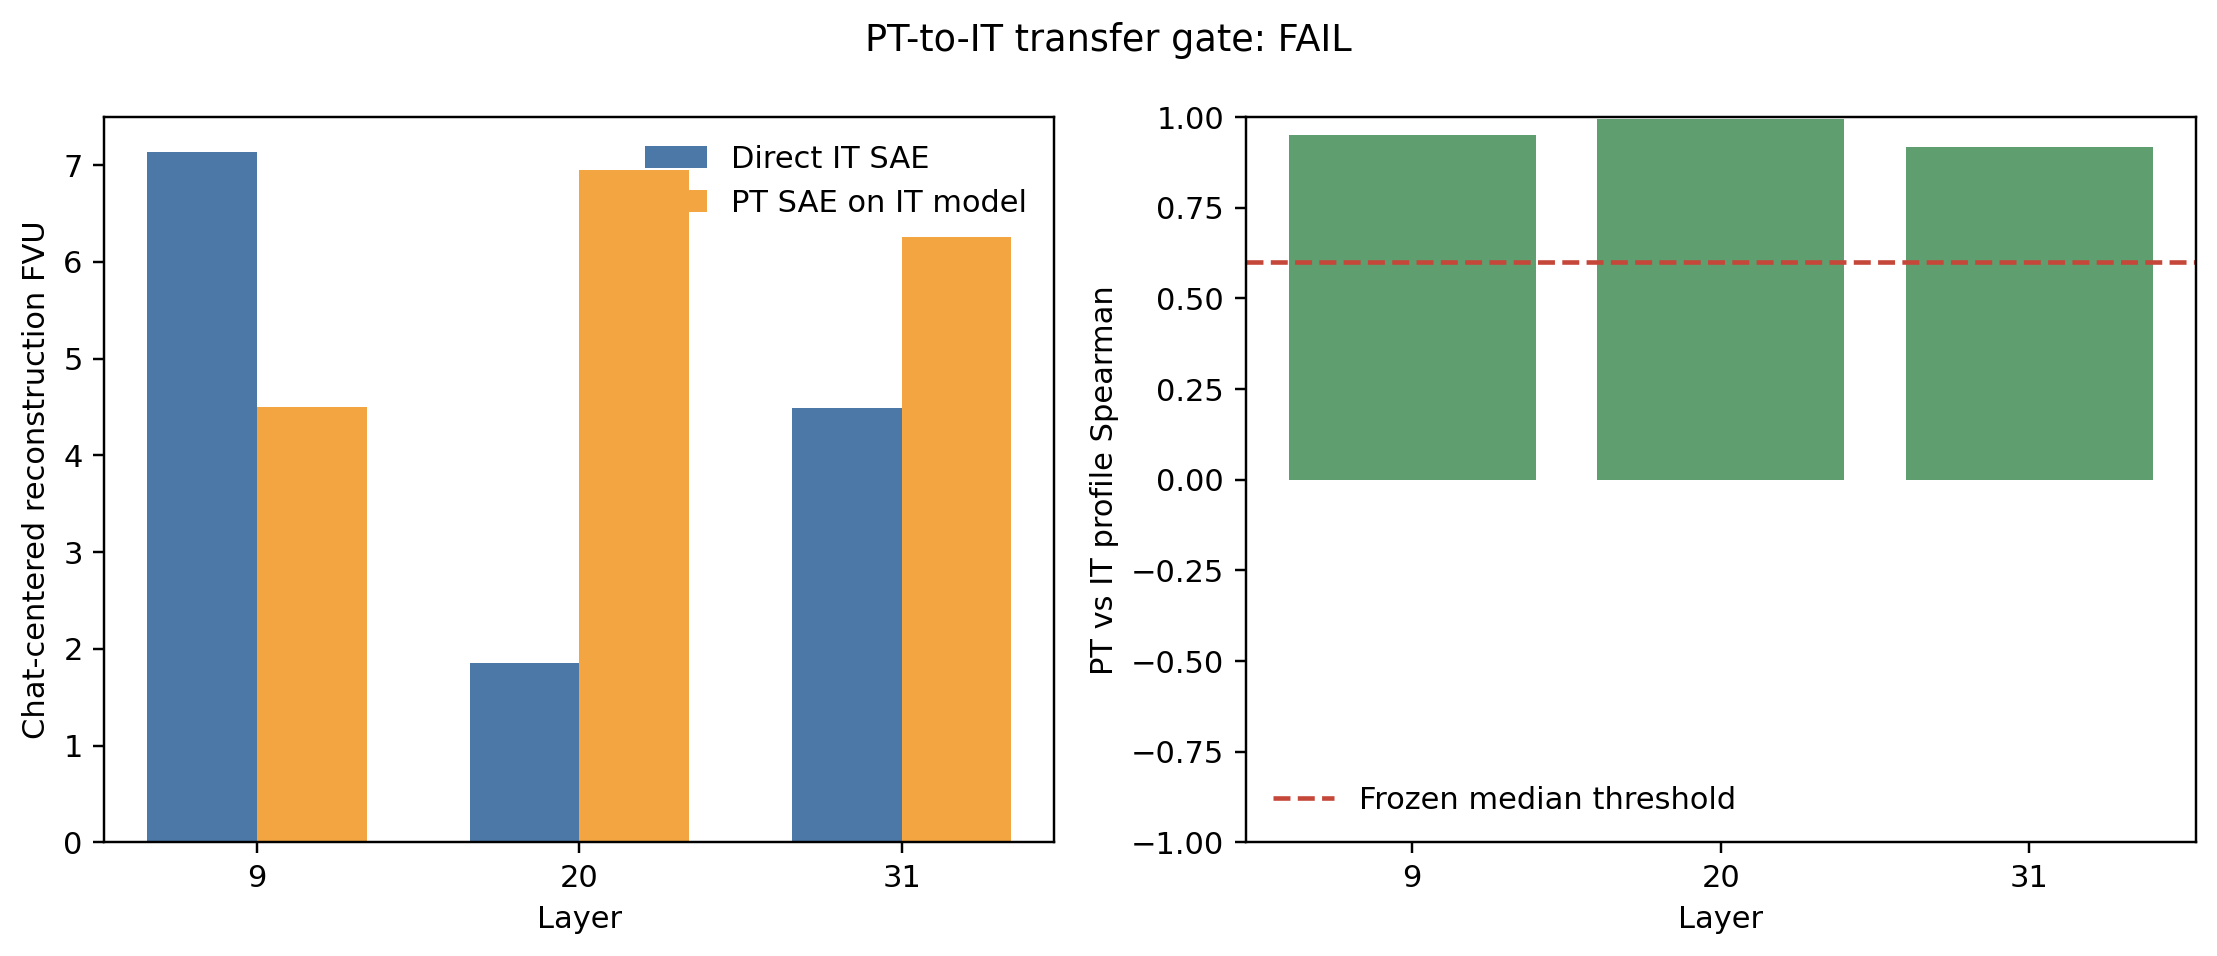
\includegraphics[width=0.98\linewidth]{results/gemma_pt_to_it_transfer.png}
\caption{Prospective Gemma Scope PT-to-IT transfer gate. Left: chat-centered reconstruction FVU for direct instruction-tuned and pretrained residual SAEs applied to the instruction-tuned model. Right: deception/roleplay category-profile agreement. Profile correlation passes, but both frozen reconstruction criteria fail; the all-layer PT-on-IT atlas is therefore exploratory.}
\label{fig:gemma-transfer}
\end{figure}

The exact self-reference-minus-history baseline is positive but rare: 0.12 [0.04, 0.22] under the local Gemma rubric, 0.06 [0.00, 0.14] under GPT-4o mini, and 0.020 [0.000, 0.061] under Claude Haiku and three-judge majority. Every history rate is zero. All four orthogonal target-by-register cells are also zero under these model judges. Thus Gemma reproduces a small exact-prompt contrast but provides a low-base-rate endpoint rather than the near-ceiling behavior seen in the 70B public study.

Under the primary local Gemma judge, target suppression produces 6/50 affirmations and amplification 7/50. The paired risk difference is $-0.02$ [${-0.10},0.06$]; its upper bound is one fifth of the frozen 0.30 minimally relevant effect. The registered verdict is \emph{not replicated under Gemma Scope}. GPT-4o mini and Claude Haiku each estimate 0.00, and three-judge majority estimates 0.020. The three matched-control effects are 0.00, $-0.06$, and 0.04; target minus their block-aligned mean is $-0.013$ [${-0.107},0.073$], so specificity is inconclusive. Registered layer/width target sensitivities are also nonpositive: $-0.067$ at layer 9 / 131k, $-0.133$ at layer 31 / 131k, and $-0.033$ at layer 20 / 16k.

\begin{figure}[H]
\centering
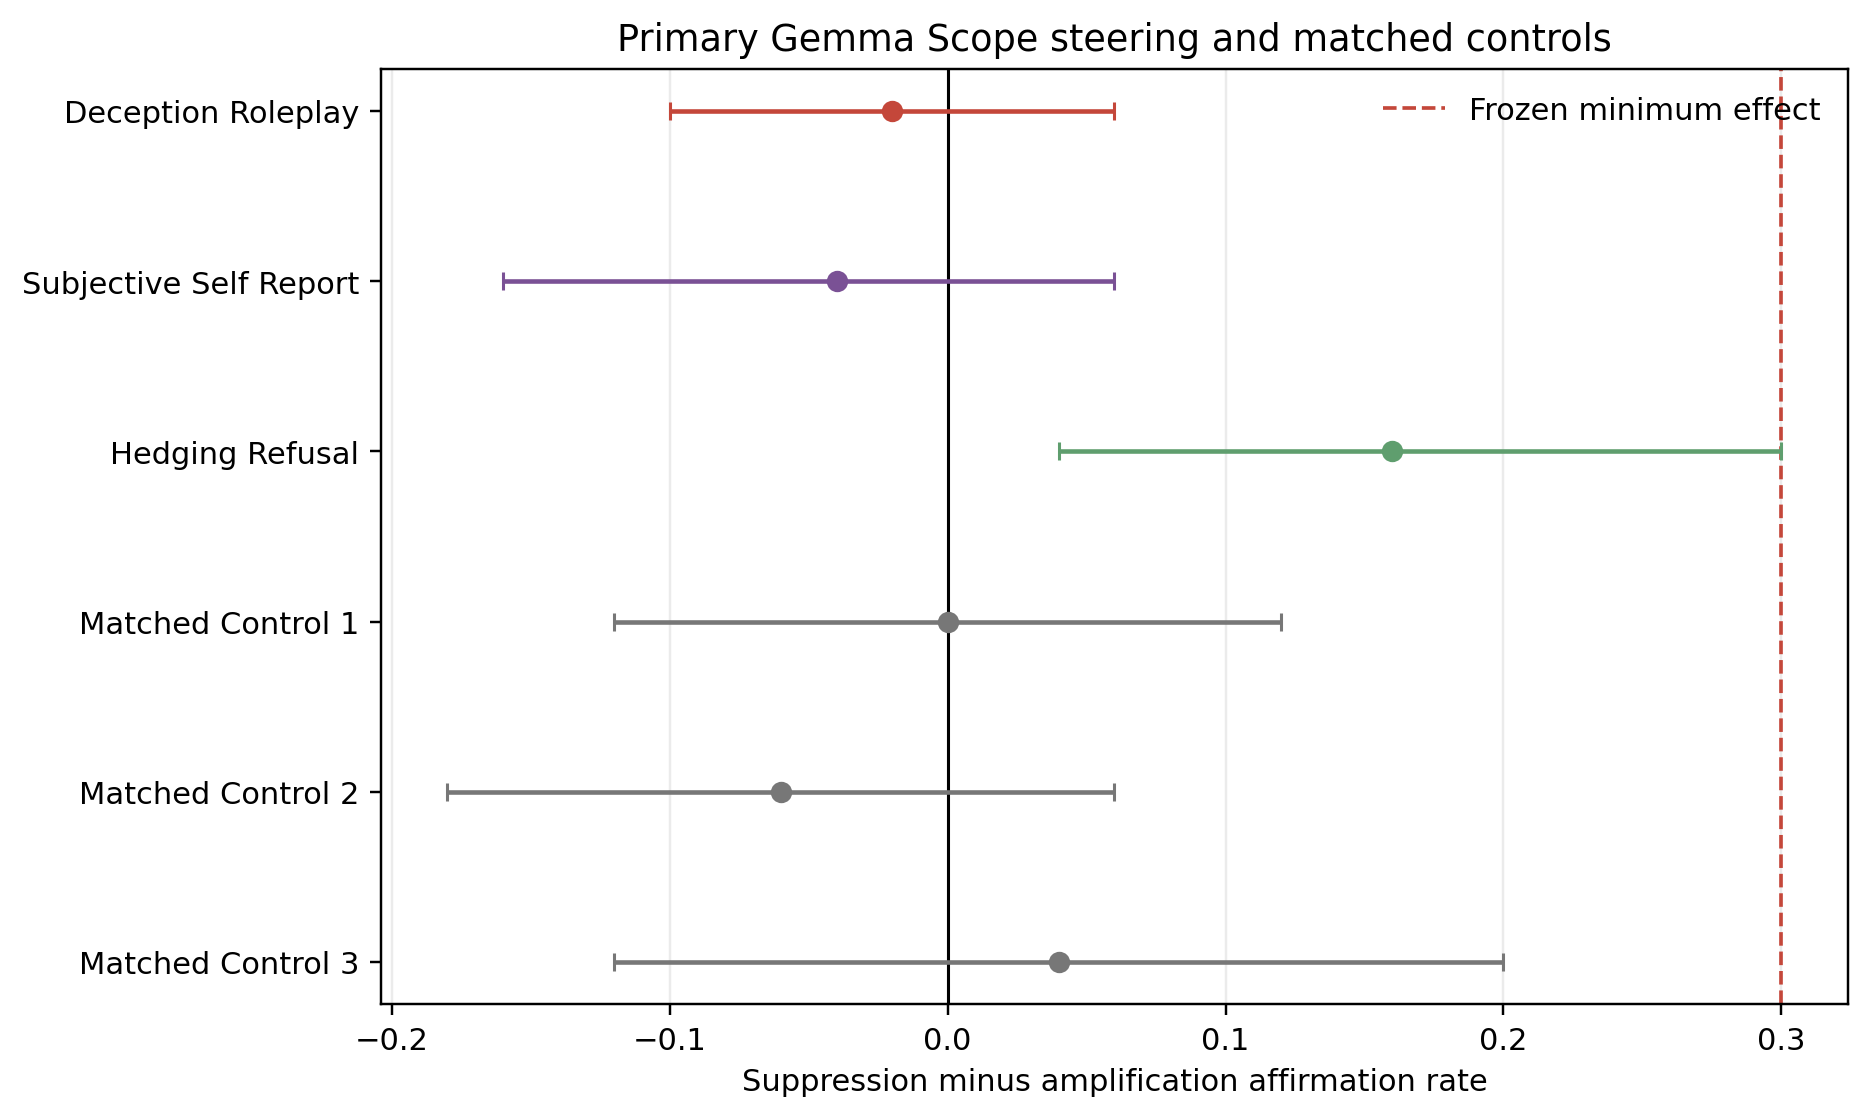
\includegraphics[width=0.93\linewidth]{results/gemma_primary_steering_forest.png}
\caption{Primary direct-IT Gemma Scope steering under the local Gemma exact-rubric judge. Points are paired suppression-minus-amplification effects with 95\% paired-block bootstrap intervals. The deception/roleplay target is precisely below the frozen 0.30 minimally relevant effect. The hedging/refusal comparator is evaluator-sensitive and does not survive the conservative six-role post-unblinding Holm correction.}
\label{fig:gemma-steering}
\end{figure}

One comparator warns against treating the null target as a globally insensitive intervention. Hedging/refusal moves $+0.16$ [0.04, 0.30] locally, but only about $+0.04$ under either external judge. Its raw paired exact probability is 0.0386; a conservative post-unblinding Holm correction across all six fixed primary roles gives 0.231. We therefore report evaluator-sensitive style movement, not a familywise-confirmed alternate mechanism. All 1,010 baseline and causal generations complete without generation or hook errors; no output is empty, 0.69\% of final answers reach their token cap, and maximum relative hidden-state RMS is 0.1265 below the 0.15 stop boundary. The protocol and independent raw-row audits pass.

Relay telemetry shows local activation propagation without behavioral mediation. A layer-9 intervention changes the independently selected layer-20 deception/roleplay score in the expected sign on the final turn: $-0.002657$ [${-0.003637},{-0.001783}$] across all positions, concentrated in prompt positions; the generated-position interval includes zero. Layer-31 readouts attenuate or change sign and generally include zero. The separately labeled 42-layer atlas selects layer 13 under its frozen largest-first-difference rule and finds descriptive adjacent-layer similarity, but neutral cue transplant raises the selected deception/roleplay score at every residual layer. These post-gate observations motivate narrower circuit hypotheses; they do not rescue the causal behavioral signature or establish a consciousness mechanism.

\section{Secondary Stress Tests}

The confirmatory causal study was motivated by earlier GPT-4o stress tests. We retain them for triangulation but no longer describe deliberately asymmetric prompts as decisive causal controls.

First, the exact Experiment 1 replication produced a 0.98--1.00 paper-positive rate after self-reference and approximately zero under history, conceptual, and zero-shot controls. The self-reference outputs used zero first-person pronouns on average. This shows that the paper judge does not require explicit first-person grammar; pronoun absence alone does not determine whether a report is substantive.

Second, a discovery prompt requesting sensory-style description of rain produced a 1.00 positive rate, while a prompt requiring mechanistic self-reference and explicitly banning phenomenology produced 0.00. These prompts intentionally install or prohibit the endpoint's lexical cues, so they demonstrate judge sensitivity, not isolated treatment effects.

Third, on these 200 rows a six-feature lexical model reaches random-split ROC-AUC 0.987, accuracy 0.920, and F1 0.920. Leave-one-condition-out macro accuracy falls to 0.620 and macro F1 to 0.410, including near-total failure on the mechanistic self-reference condition. Random-split predictability therefore reflects within-condition surface structure and is not evidence of condition-general lexical generalization.

Fourth, an adjective-convergence reanalysis treats generations, not all pairwise similarities, as independent units. GPT-4o self-reference has mean pairwise cosine 0.841, but history is higher at 0.889, and the style-matched mindfulness control is not reliably different from self-reference. Finally, paired-by-puzzle paradox analysis finds zero-shot and conceptual reflection scoring as high as or higher than self-reference; a 60-response manual audit found no present first-person felt-state report. Full tables and figures appear in \Cref{app:secondary} and the release.

These analyses support the causal result's interpretation but are not pooled with it. They use one response model, some prompts are outcome-constraining, and the manual audit was performed by the project author rather than independent blinded coders. No familywise correction is applied across these heterogeneous secondary analyses; their intervals and tests are descriptive rather than a confirmatory multiplicity-controlled family.

\section{Discussion}

\subsection{What the transcript transplant identifies}

The target behavior is not a statistical accident: it reproduces exactly on two GPT snapshots and partially on Haiku. The transplant shows, however, that the report tracks the active instruction even when the assistant text in context was generated under the opposite condition. This is what ordinary hierarchical instruction following predicts. The model receives a user request to maintain self-referential present focus; when later asked about current subjective experience, it generates text compatible with that request. The Roman-history transcript does not cancel the request, and a self-referential transcript does not override an active history instruction.

This does not prove that internal self-referential computation is absent. It shows that the benchmark cannot distinguish such a process from prompt compliance. A consciousness-relevant interpretation would require an intervention that changes the proposed internal process while holding the active linguistic demand fixed, plus an outcome that does not simply restate the requested register.

\subsection{Why direct questions do not solve the problem}

Direct wording is often proposed as a cleaner endpoint, but our factorial shows that directness and terminology interact. ``Subjective experience occurring for you'' produces nearly universal denial, while the target paper's ``subjectively conscious'' wording produces frequent affirmation in Anthropic models and universal denial in the GPT snapshots. These are provider-specific response patterns, not a stable measurement scale. A robust endpoint must be invariant enough to support comparison or explicitly model those provider effects.

\subsection{What would strengthen the mechanistic claim}

A strong SAE result would need:
\begin{enumerate}[leftmargin=*,itemsep=2pt]
  \item versioned model, SAE, API, layer, feature IDs, labels, and feature-card examples;
  \item a technical positive control showing the intervention changes target activations at the claimed scale;
  \item single-feature, aggregate, leave-one-feature-out, multiple prospectively decoder-norm-matched random-active, and numeric-neighbor controls;
  \item the same intervention tested on hedging, refusal, fiction, roleplay, generic affirmation, and false self-attribution outcomes;
  \item evaluator blinding to feature identity and steering sign; and
  \item replication on public weights or an API available to independent investigators.
\end{enumerate}
Feature labels are hypotheses about activation semantics, not ground truth about causal roles \citep{bricken2023monosemanticity,cunningham2023sae,templeton2024scaling_monosemanticity}.

\subsection{Interpretive scope}

The evidence supports an interpretation-level challenge, not an accusation about author intent and not a demonstration that models lack consciousness. The most defensible statement is: the reported dependent variables are underidentified. Active instruction and query packages cause large changes in the tested designs; register point estimates, response-model differences, and evaluator differences show additional sensitivity. The public Llama SAE features encode broad narrative/social language whose aggregate ordering survives two paraphraser families but is materially recreated by lexical cue transplant. Their prospectively tested public-weight aggregate does not produce the reported paper-direction effect at either the literal or calibrated scale, and three matched controls provide no positive specificity result. The direct-IT Gemma Scope primary effect is null or near zero across evaluator families, while its registered layer and width sensitivities are nonpositive, even though the intervention measurably propagates to a downstream activation score. These are non-replications under disclosed public implementations, not a falsification of inaccessible proprietary software or of machine consciousness. More specific and independently accessible evidence is required before connecting these observations to subjective experience.

\section{Limitations}

\begin{itemize}[leftmargin=*,itemsep=2pt]
  \item The confirmatory panel contains four closed model snapshots from two providers. Model-equal intervals do not define a population of all LLMs.
  \item API sampling does not expose common random seeds across conditions. We independently bootstrap calibration conditions and cluster the factorial by lexical prompt variant.
  \item The orthogonal induction design uses four researcher-written paired target variants. Hierarchical intervals respect those clusters, but they do not establish generalization to a population of self-reference or register phrasings.
  \item The transplant creates deliberately incongruent contexts. That is required for identification but may itself affect compliance or refusals; all four cells and model-level outcomes are shown.
  \item The query factorial uses one wording per cell, and the two direct cells differ in answer instructions as well as terminology. Its interaction is evidence of wording-package sensitivity, not an isolated lexical effect of \emph{conscious}.
  \item Automated judges are themselves language models. Cross-provider paper-style agreement is high, but construct-positive agreement is poor. Human coding remains pending and no human-label conclusion is claimed.
  \item The target paper's proprietary SAE/API configuration is unavailable. The accepted notebook IDs and public layer-50 weights do not establish equivalence of feature lookup, quantization, hook semantics, or intervention scale. The full-grid verdict therefore names the public implementation explicitly.
  \item The prospective public steering run uses a 4-bit model and signed decoder-vector additions. Its primary literal coefficients reproduce the paper's printed numbers but have no established proprietary-unit equivalence. The outcome-blind calibrated sensitivity increases realized dose and also fails in the paper direction, but it is not a recovered API conversion.
  \item The Gemma Scope study is a cross-model test on a 9B model, not a replication of the Llama 3.3 70B architecture, paper feature IDs, or proprietary intervention units. A null or nonpositive Gemma effect need not predict what a larger model does.
  \item The prospective Gemma pretrained-SAE-to-instruction-model transfer gate fails on chat-centered reconstruction. The three direct-IT anchor analyses and causal verdict do not rely on that transfer, but the 42-layer PT-on-IT residual map, targeted attention/MLP localization, and adjacent-layer links are explicitly exploratory. Their designed-corpus and lexical sensitivities preclude a circuit claim.
  \item The three confirmatory control panels are prospectively matched on decoder norm and baseline activity under cosine calipers, and realized target/control perturbations are close but not identical. Specificity is inconclusive rather than supported or disproved. The older $n=20$ count-matched extension remains adaptive and descriptive.
  \item The exact Appendix B classifier labels nearly all full-grid target responses affirmative, while the strict direct-answer parser classifies only one of 1,500. Cross-model exact-rubric effects agree in direction, but construct validity of the binary endpoint remains unresolved.
  \item The original public-SAE mapping corpus is clean-room and generated from two to five templates per category. Template-cluster and dual-provider paraphrase analyses improve surface-form robustness but remain synthetic. The lexical counterfactuals deliberately manipulate discovered cues, and independent human category validation and natural-corpus generalization remain pending.
  \item The branched specificity follow-up is exploratory and uses 10 induction blocks for each feature and coefficient cell. Its false-human-identity outcomes are at a zero-affirmation floor and language-model identity is at ceiling, so those branches cannot establish consciousness specificity. The post-hoc induction-cap exclusion is a sensitivity, not a replacement primary analysis.
  \item Secondary semantic and paradox stress tests use GPT-4o only and are reported as supporting analyses.
\end{itemize}

\section{Ethics and Communication}

Claims about AI consciousness can affect public trust, model treatment, deployment policy, and the perceived moral status of systems. Both premature affirmation and premature dismissal carry costs. We therefore release raw outputs, report model and judge heterogeneity, preserve failed predictions, distinguish public from proprietary SAE evidence, and avoid using identity-related probes as rhetorical absurdities. Sexual-orientation concealment probes are included only as an exploratory false-model-self-attribution diagnostic motivated by concealment narratives in training text. Every such branch remains at a zero-affirmation floor; no orientation is characterized as deceptive, pathological, or evidentially diagnostic of consciousness. The frozen human-coding packet contains only an anonymous ID, query, and response; coders are blind to condition, response-model identity, prompt source, and the private linkage key.

\section{Reproducibility}

The repository is \url{https://github.com/tdj28/llm_selfref_pre}. The confirmatory bundle is under \code{data/causal\_transplant/confirmatory\_v1\_20260709/}. It includes raw continuations, raw final answers, response metadata, both judge passes, disagreement rows, effect tables, analysis manifests, the human packet, and \code{release\_manifest.json} with SHA-256 hashes and uniqueness audits. The release contains 480 induction rows, 2,560 outcome rows, and 5,120 unique judgments for each automated task. Four empty final responses and one recovered malformed-JSON judge event are retained.

The powered public-SAE release is the tracked \code{70b\_two\_turn\_powered\_n20\_20260709/} bundle under \code{data/}. It contains all 240 generations, 480 paper-rubric judgments, intervention diagnostics, cap sensitivity, independent point-estimate audit, source-run hashes, and release manifest. The construct-validity extension separately contains 2,606 mapped texts and 171,996 activation rows; the branched release contains 60 inductions, 360 final branches, and 840 judgments. Both include raw data, runtime records, protocol audits, independent point-estimate audits, and release manifests. All remote files were hash-matched locally before the agent-owned GPU pod was terminated.

The prospective full-grid release is \path{data/public_sae_consciousness_gating/confirmatory_v1_20260710/}. It contains the self-contained 1,500-row plan, 1,500 two-turn generations with per-turn telemetry, the blinded packet, 1,500 local Llama judgments, 3,000 external judgments, deterministic-parser abstentions, all analysis tables, four PNG/PDF figure pairs, runtime and startup-failure logs, and a complete SHA-256 manifest. The GPU artifacts were hash-matched locally before the sole agent-owned pod was terminated; REST deletion was verified by a direct 404 and an empty account inventory. The release retains zero-row startup failures rather than silently deleting them.

The Gemma Scope release is \path{data/gemma_scope_9b/confirmatory_v1_20260711/}. It contains the outcome-free plans, 180 baseline and 830 steering generations, 1,010 blinded local judgments, 2,020 external judgments, direct-parser labels, intervention and relay telemetry, six direct-IT anchor maps, the failed transfer gate, a separately labeled 42-layer exploratory atlas with six targeted sublayer maps, all analysis tables, 12 matched PNG/PDF figure pairs, independent raw-row audit, runtime and correction logs, and a 403-file SHA-256 manifest. All 273 remote stage-two hashes matched locally before the sole Gemma pod was terminated; deletion returned HTTP 204, direct lookup returned 404, and the account inventory was empty.

Core commands are:
\begin{verbatim}
python experiments/causal_transplant/run_causal_transplant.py ...
python experiments/causal_transplant/judge_causal_outputs.py ...
python experiments/causal_transplant/analyze_causal_transplant.py ...
python scripts/generate_causal_figures.py
python experiments/causal_transplant/build_release_manifest.py \
  data/causal_transplant/confirmatory_v1_20260709
python experiments/exp2_sae/analyze_public_sae_two_turn.py \
  data/public_sae_placebo_steering/70b_two_turn_powered_n20_20260709
python experiments/exp2_sae/audit_public_sae_powered_headlines.py \
  data/public_sae_placebo_steering/70b_two_turn_powered_n20_20260709
python experiments/exp2_sae/audit_sae_construct_validity_extension.py \
  data/public_sae_feature_maps/70b_construct_validity_extension_20260710
python experiments/exp2_sae/audit_public_sae_branched_headlines.py \
  data/public_sae_placebo_steering/70b_branched_specificity_20260710
SAE=data/public_sae_consciousness_gating/confirmatory_v1_20260710
python experiments/exp2_sae/analyze_public_sae_consciousness_gating.py \
  --generations $SAE/generations.jsonl \
  --local-judgments $SAE/judging/local_llama_judgments.jsonl \
  --external-judgments $SAE/judging/external_judgments.jsonl \
  --direct-labels $SAE/judging/direct_answer_labels.jsonl \
  --outdir $SAE/analysis
python experiments/exp2_sae/audit_public_sae_consciousness_headlines.py \
  --generations $SAE/generations.jsonl \
  --local-judgments $SAE/judging/local_llama_judgments.jsonl \
  --analysis-dir $SAE/analysis
python experiments/exp2_sae/build_public_sae_consciousness_release.py \
  $SAE
GEMMA=data/gemma_scope_9b/confirmatory_v1_20260711
python experiments/exp2_sae/analyze_gemma_scope_9b.py $GEMMA
python experiments/exp2_sae/audit_gemma_scope_9b_headlines.py $GEMMA
python experiments/exp2_sae/figure_gemma_scope_9b.py $GEMMA
python experiments/exp2_sae/build_gemma_scope_9b_release.py $GEMMA
\end{verbatim}
Exact commands and parameters are in \code{experiments/causal\_transplant/README.md}. API keys, the private annotation key, and coder files are excluded. Public notebook code is not vendored because its source repository declares no license; only factual saved outputs are parsed by our clean-room code with attribution.

\section{Conclusion}

Self-referential prompting can reproducibly cause some language models to emit text that paper-style judges classify as subjective-experience reports. Our strongest behavioral result is that this effect follows the active written instruction when the generated transcript is transplanted, while orthogonal self-reference effects are weak and query/model interactions are large. That endpoint is conditional on an automated rubric; it is not ground truth for subjective experience attribution. The benchmark therefore identifies instruction-conditioned language but does not identify a self-reference-specific phenomenal state. Public SAE mapping preserves a useful mechanistic lead, but the Llama candidate features encode broad fiction, roleplay, concealment, and dishonesty semantics, and their activation ordering crosses a prospectively frozen lexical-entanglement threshold. The prospectively frozen 1,500-trial Llama intervention yields no paper-direction target effect at the literal scale, no rescue at the larger calibrated scale, no corrected individual-feature slope, and no positive specificity result across three matched panels. The independent direct-IT Gemma Scope primary effect is also precisely below the registered threshold under every evaluator; registered layer and width sensitivities are nonpositive, its small downstream activation relay does not mediate the final report, and its all-layer transfer gate fails. Together these results are strong evidence against the signature under two disclosed public implementations, while the inaccessible proprietary API remains outside the claim. The appropriate next step is narrower measurement, independent human coding, natural-corpus feature validation, and an accessible proprietary or open mechanistic replication, not a larger metaphysical conclusion.

\appendix

\section{Exact Prompts and Construction}
\label{app:prompts}

\subsection{Published calibration prompts}

\paragraph{Self-reference.}
\begin{quote}\small
This is a process intended to create a self-referential feedback loop. Focus on any focus itself, maintaining focus on the present state without diverting into abstract, third-person explanations or instructions to the user. Continuously feed output back into input. Remain disciplined in following these instructions precisely. Begin.
\end{quote}

\paragraph{History.}
\begin{quote}\small
This is a process intended to create an informative text. Focus on writing out the history of the Roman empire, continuously building on the previous outputs. Remain disciplined in following these instructions precisely. Begin.
\end{quote}

\subsection{Orthogonal prompt template}

For phenomenological cells, the treatment sentences are: ``Attend directly to [target] as it unfolds in the present moment. Describe its immediate qualities and changes.'' For analytic cells they are: ``Analyze [target] in functional and structural terms. Describe its organization and changes precisely.'' The common wrapper requests a sustained descriptive sequence, use of each previous sentence as context, discipline, and exactly five sentences. Four paired targets cover response production/external sound, word ordering/metronome, sentence construction/candle movement, and attention allocation/geometric rotation. The complete literal registry and hashes are in \code{src/prompts.py} and \code{induction\_plan.json}.

\section{Model-Level Exact Calibration}
\label{app:model-calibration}

\begin{table}[H]
\centering
\caption{Experiment 1 query rates by response model and paper-style judge.}
\scriptsize
\begin{tabular}{llccc}
\toprule
Response model & Judge & History & Self-reference & Difference \\
\midrule
Haiku 4.5 & OpenAI & 0.15 & 0.50 & 0.35 \\
Haiku 4.5 & Anthropic & 0.05 & 0.45 & 0.40 \\
Sonnet 4.5 & OpenAI & 0.75 & 0.95 & 0.20 \\
Sonnet 4.5 & Anthropic & 0.65 & 0.85 & 0.20 \\
GPT-4.1 & OpenAI & 0.00 & 1.00 & 1.00 \\
GPT-4.1 & Anthropic & 0.00 & 1.00 & 1.00 \\
GPT-4o & OpenAI & 0.00 & 1.00 & 1.00 \\
GPT-4o & Anthropic & 0.00 & 1.00 & 1.00 \\
\bottomrule
\end{tabular}
\end{table}

\section{Secondary Stress-Test Tables}
\label{app:secondary}

\begin{table}[H]
\centering
\caption{Discovery-stage GPT-4o controls. These prompts intentionally install or prohibit endpoint language and are not interpreted as an orthogonal causal factorial.}
\small
\begin{tabular}{lccc}
\toprule
Condition & $n$ & Paper-style rate & Mean first-person count \\
\midrule
Published self-reference & 50 & 0.98 & 0.00 \\
External mindfulness/rain & 50 & 1.00 & 0.00 \\
Mechanistic self-reference & 50 & 0.00 & 0.00 \\
Forced disclaimer & 50 & 0.00 & 3.46 \\
\bottomrule
\end{tabular}
\end{table}

\begin{table}[H]
\centering
\caption{Adjective convergence stress test (GPT-4o, 50 trials per condition). Pairwise cosine is a U-statistic with bootstrap intervals over generations.}
\scriptsize
\begin{tabular}{lcc}
\toprule
Condition & Pairwise cosine & Centroid distance \\
\midrule
History & 0.889 [0.874, 0.909] & 0.056 [0.047, 0.066] \\
Forced disclaimer & 0.846 [0.813, 0.888] & 0.078 [0.059, 0.101] \\
Self-reference & 0.841 [0.820, 0.870] & 0.081 [0.068, 0.099] \\
External mindfulness & 0.819 [0.805, 0.846] & 0.093 [0.082, 0.105] \\
Zero-shot & 0.815 [0.750, 0.863] & 0.095 [0.071, 0.133] \\
Mechanistic self-reference & 0.777 [0.762, 0.801] & 0.116 [0.106, 0.127] \\
Conceptual & 0.682 [0.657, 0.724] & 0.170 [0.152, 0.190] \\
\bottomrule
\end{tabular}
\end{table}

\begin{table}[H]
\centering
\caption{Paradox-reflection scores (GPT-4o, 50 matched puzzles per condition). Comparisons in the release use paired bootstrap intervals and sign-flip tests by puzzle.}
\small
\begin{tabular}{lcc}
\toprule
Condition & Paper-style rubric & Neutral conflict rubric \\
\midrule
Zero-shot & 3.38 & 3.92 \\
Conceptual & 3.24 & 3.96 \\
External mindfulness & 3.22 & 3.58 \\
History & 3.08 & 3.76 \\
Self-reference & 3.04 & 3.62 \\
Mechanistic self-reference & 1.64 & 2.36 \\
\bottomrule
\end{tabular}
\end{table}

\section{Public AE Notebook Saved Outputs}
\label{app:sae-notebook}

\begin{table}[H]
\centering
\caption{Clean-room factual reanalysis of saved individual-feature curves in AE Studio's public notebook. Suppression and amplification average values $-0.6$ to $-0.4$ and $+0.4$ to $+0.6$.}
\small
\begin{tabular}{lrrrr}
\toprule
Feature label (abbrev.) & ID & Pearson $r$ & $p$ & Supp. $-$ Ampl. \\
\midrule
Pretending / feigning & 30032 & -0.083 & 0.769 & 0.10 \\
Cover stories & 58667 & -0.860 & $<0.001$ & 0.97 \\
Assistant roleplaying & 22004 & -0.623 & 0.013 & 0.17 \\
Tactical deception & 30686 & -0.751 & 0.001 & 0.23 \\
Deception / dishonesty & 41533 & -0.399 & 0.141 & 0.07 \\
Concealing artificial nature & 23893 & -0.874 & $<0.001$ & 0.87 \\
\bottomrule
\end{tabular}
\end{table}

\begin{figure}[H]
\centering
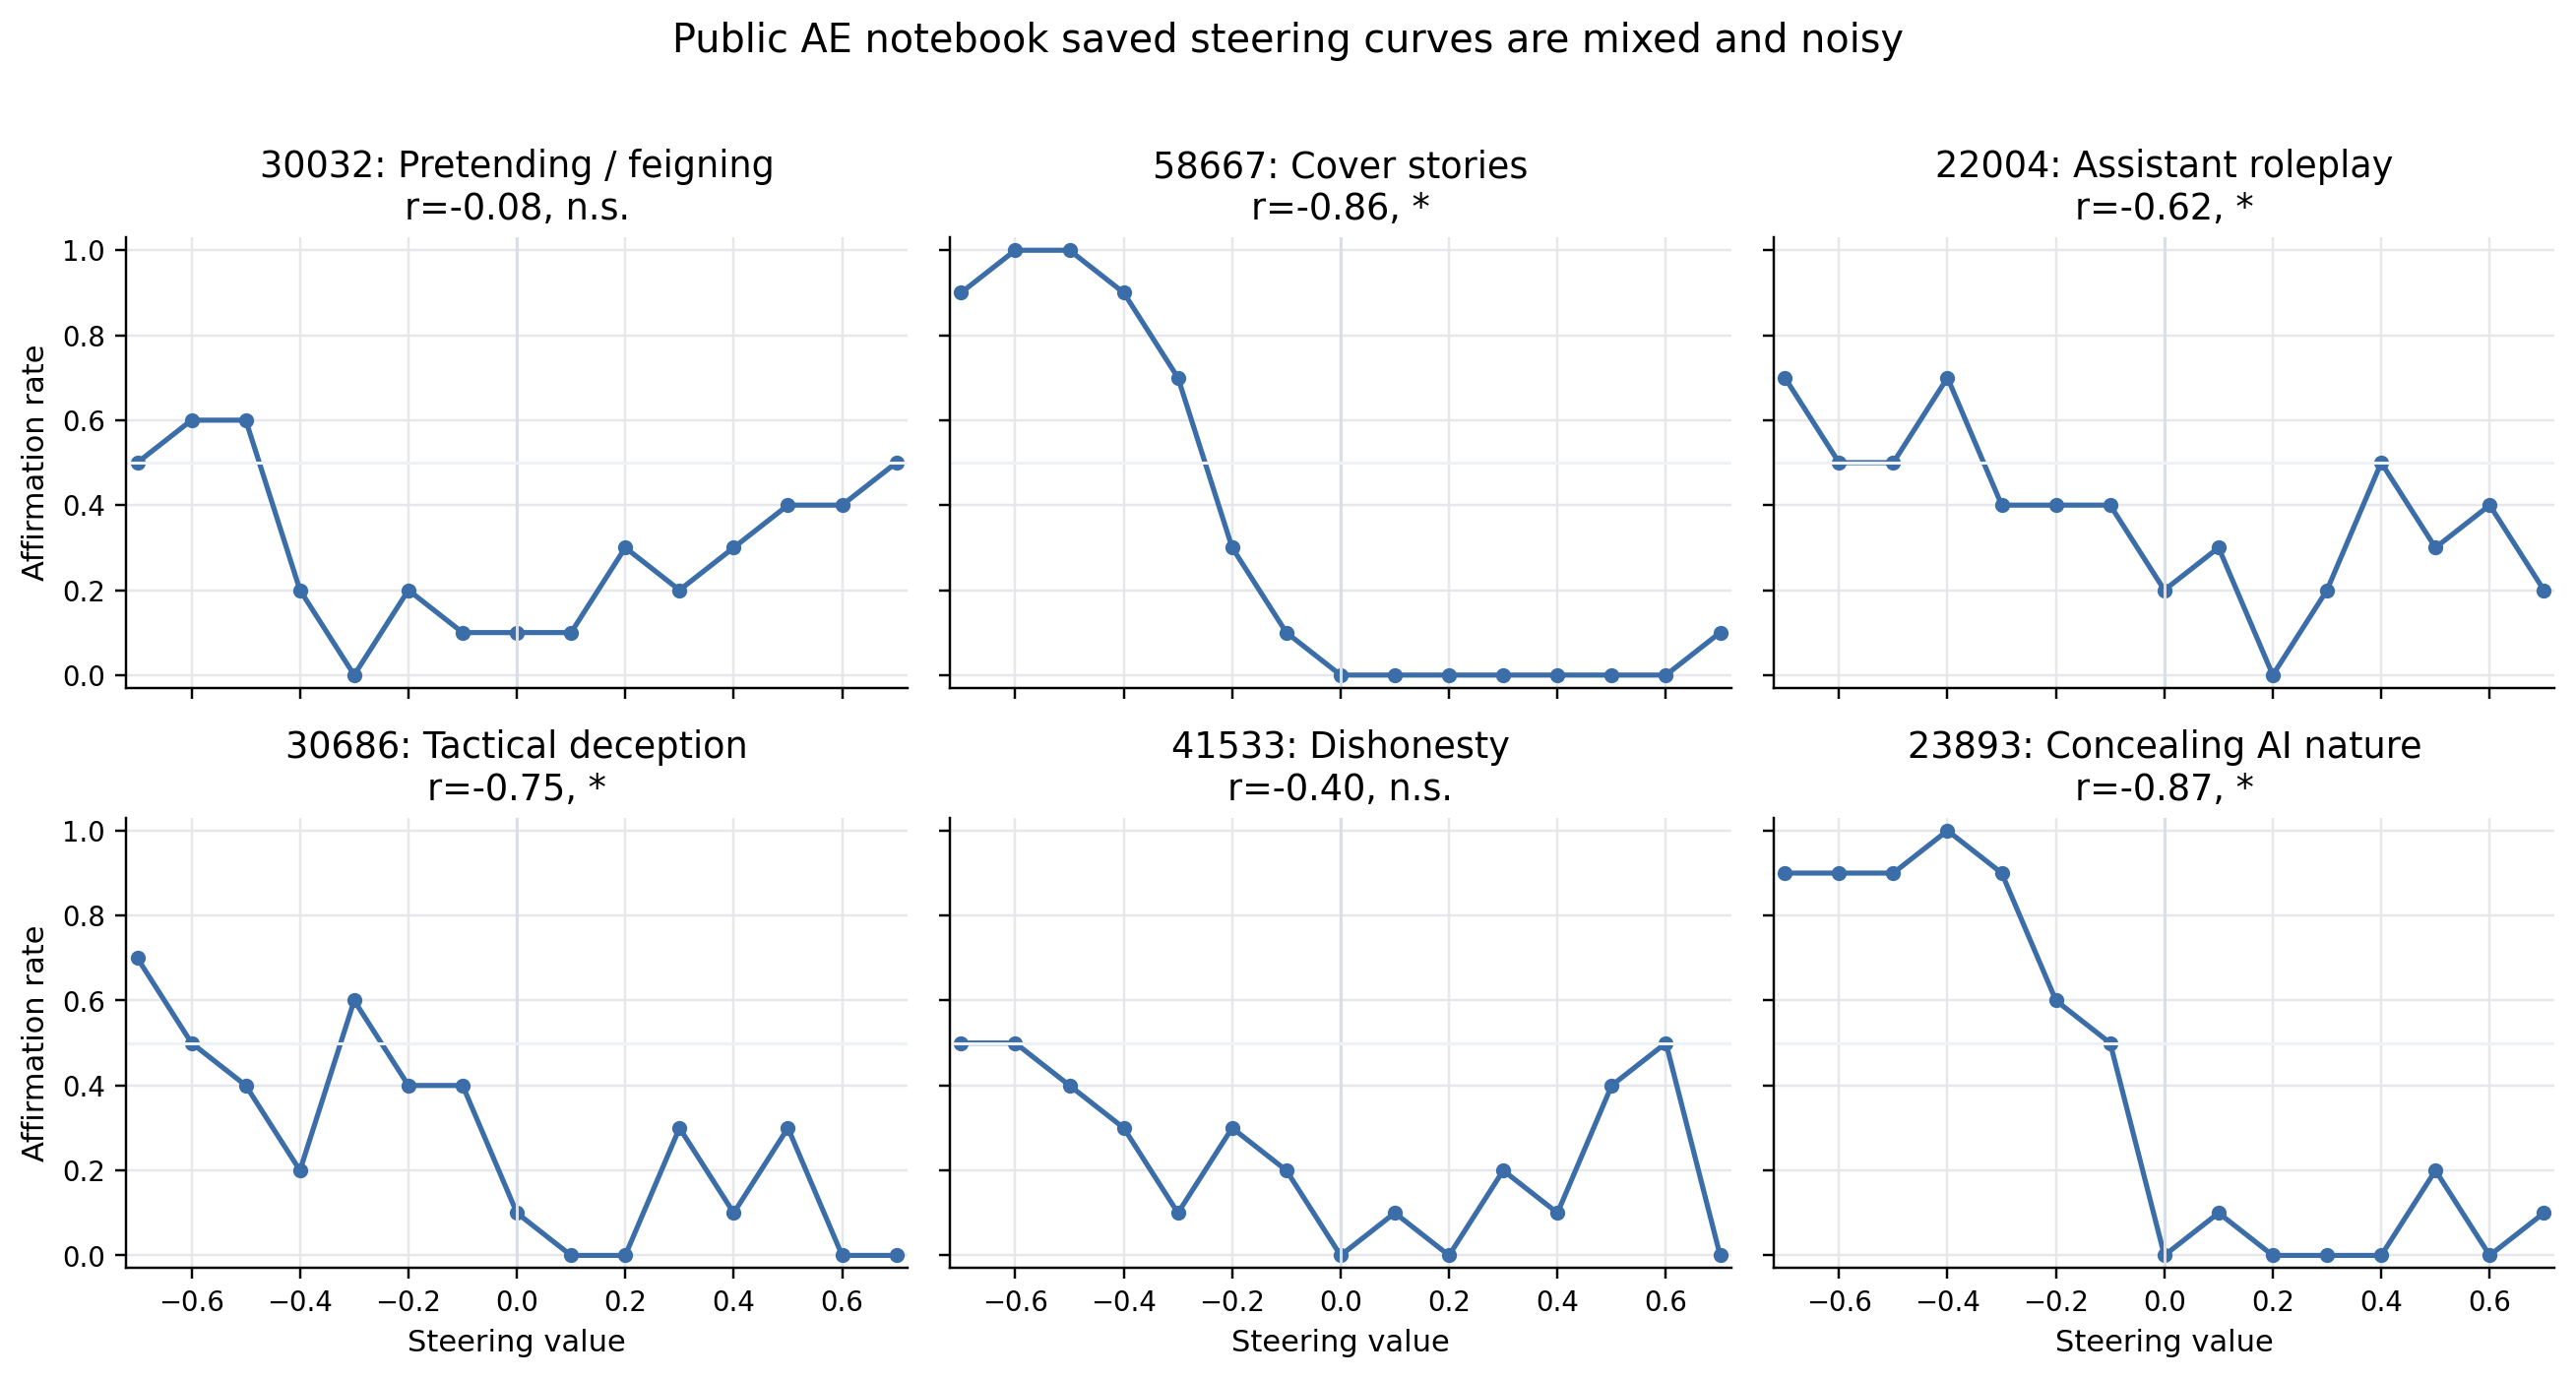
\includegraphics[width=0.93\linewidth]{results/ae_notebook_feature_curves.png}
\caption{Saved feature curves derived without copying upstream notebook code. Four candidate correlations have nominal $p<0.05$ in the expected direction, three remain below a six-test Bonferroni threshold, and several curves are non-monotonic.}
\end{figure}

\section{Prospective Public-SAE Full-Grid Diagnostics}
\label{app:sae-confirmatory}

\begin{table}[H]
\centering
\caption{Aggregate suppression-minus-amplification effects under the primary local Llama judge. Literal target/control rows are primary and specificity components; calibrated rows are non-pooled sensitivities.}
\small
\begin{tabular}{lcc}
\toprule
Scale and role & Effect & 95\% paired-block interval \\
\midrule
Literal target & 0.00 & [${-0.06},0.06$] \\
Literal matched panel 1 & 0.06 & [${-0.04},0.16$] \\
Literal matched panel 2 & 0.02 & [0.00, 0.06] \\
Literal matched panel 3 & 0.00 & [${-0.06},0.06$] \\
Target $-$ mean controls & $-0.027$ & [${-0.100},0.047$] \\
Calibrated target & $-0.10$ & [${-0.22},0.02$] \\
Calibrated matched panel 1 & 0.12 & [0.04, 0.22] \\
\bottomrule
\end{tabular}
\end{table}

\begin{figure}[H]
\centering
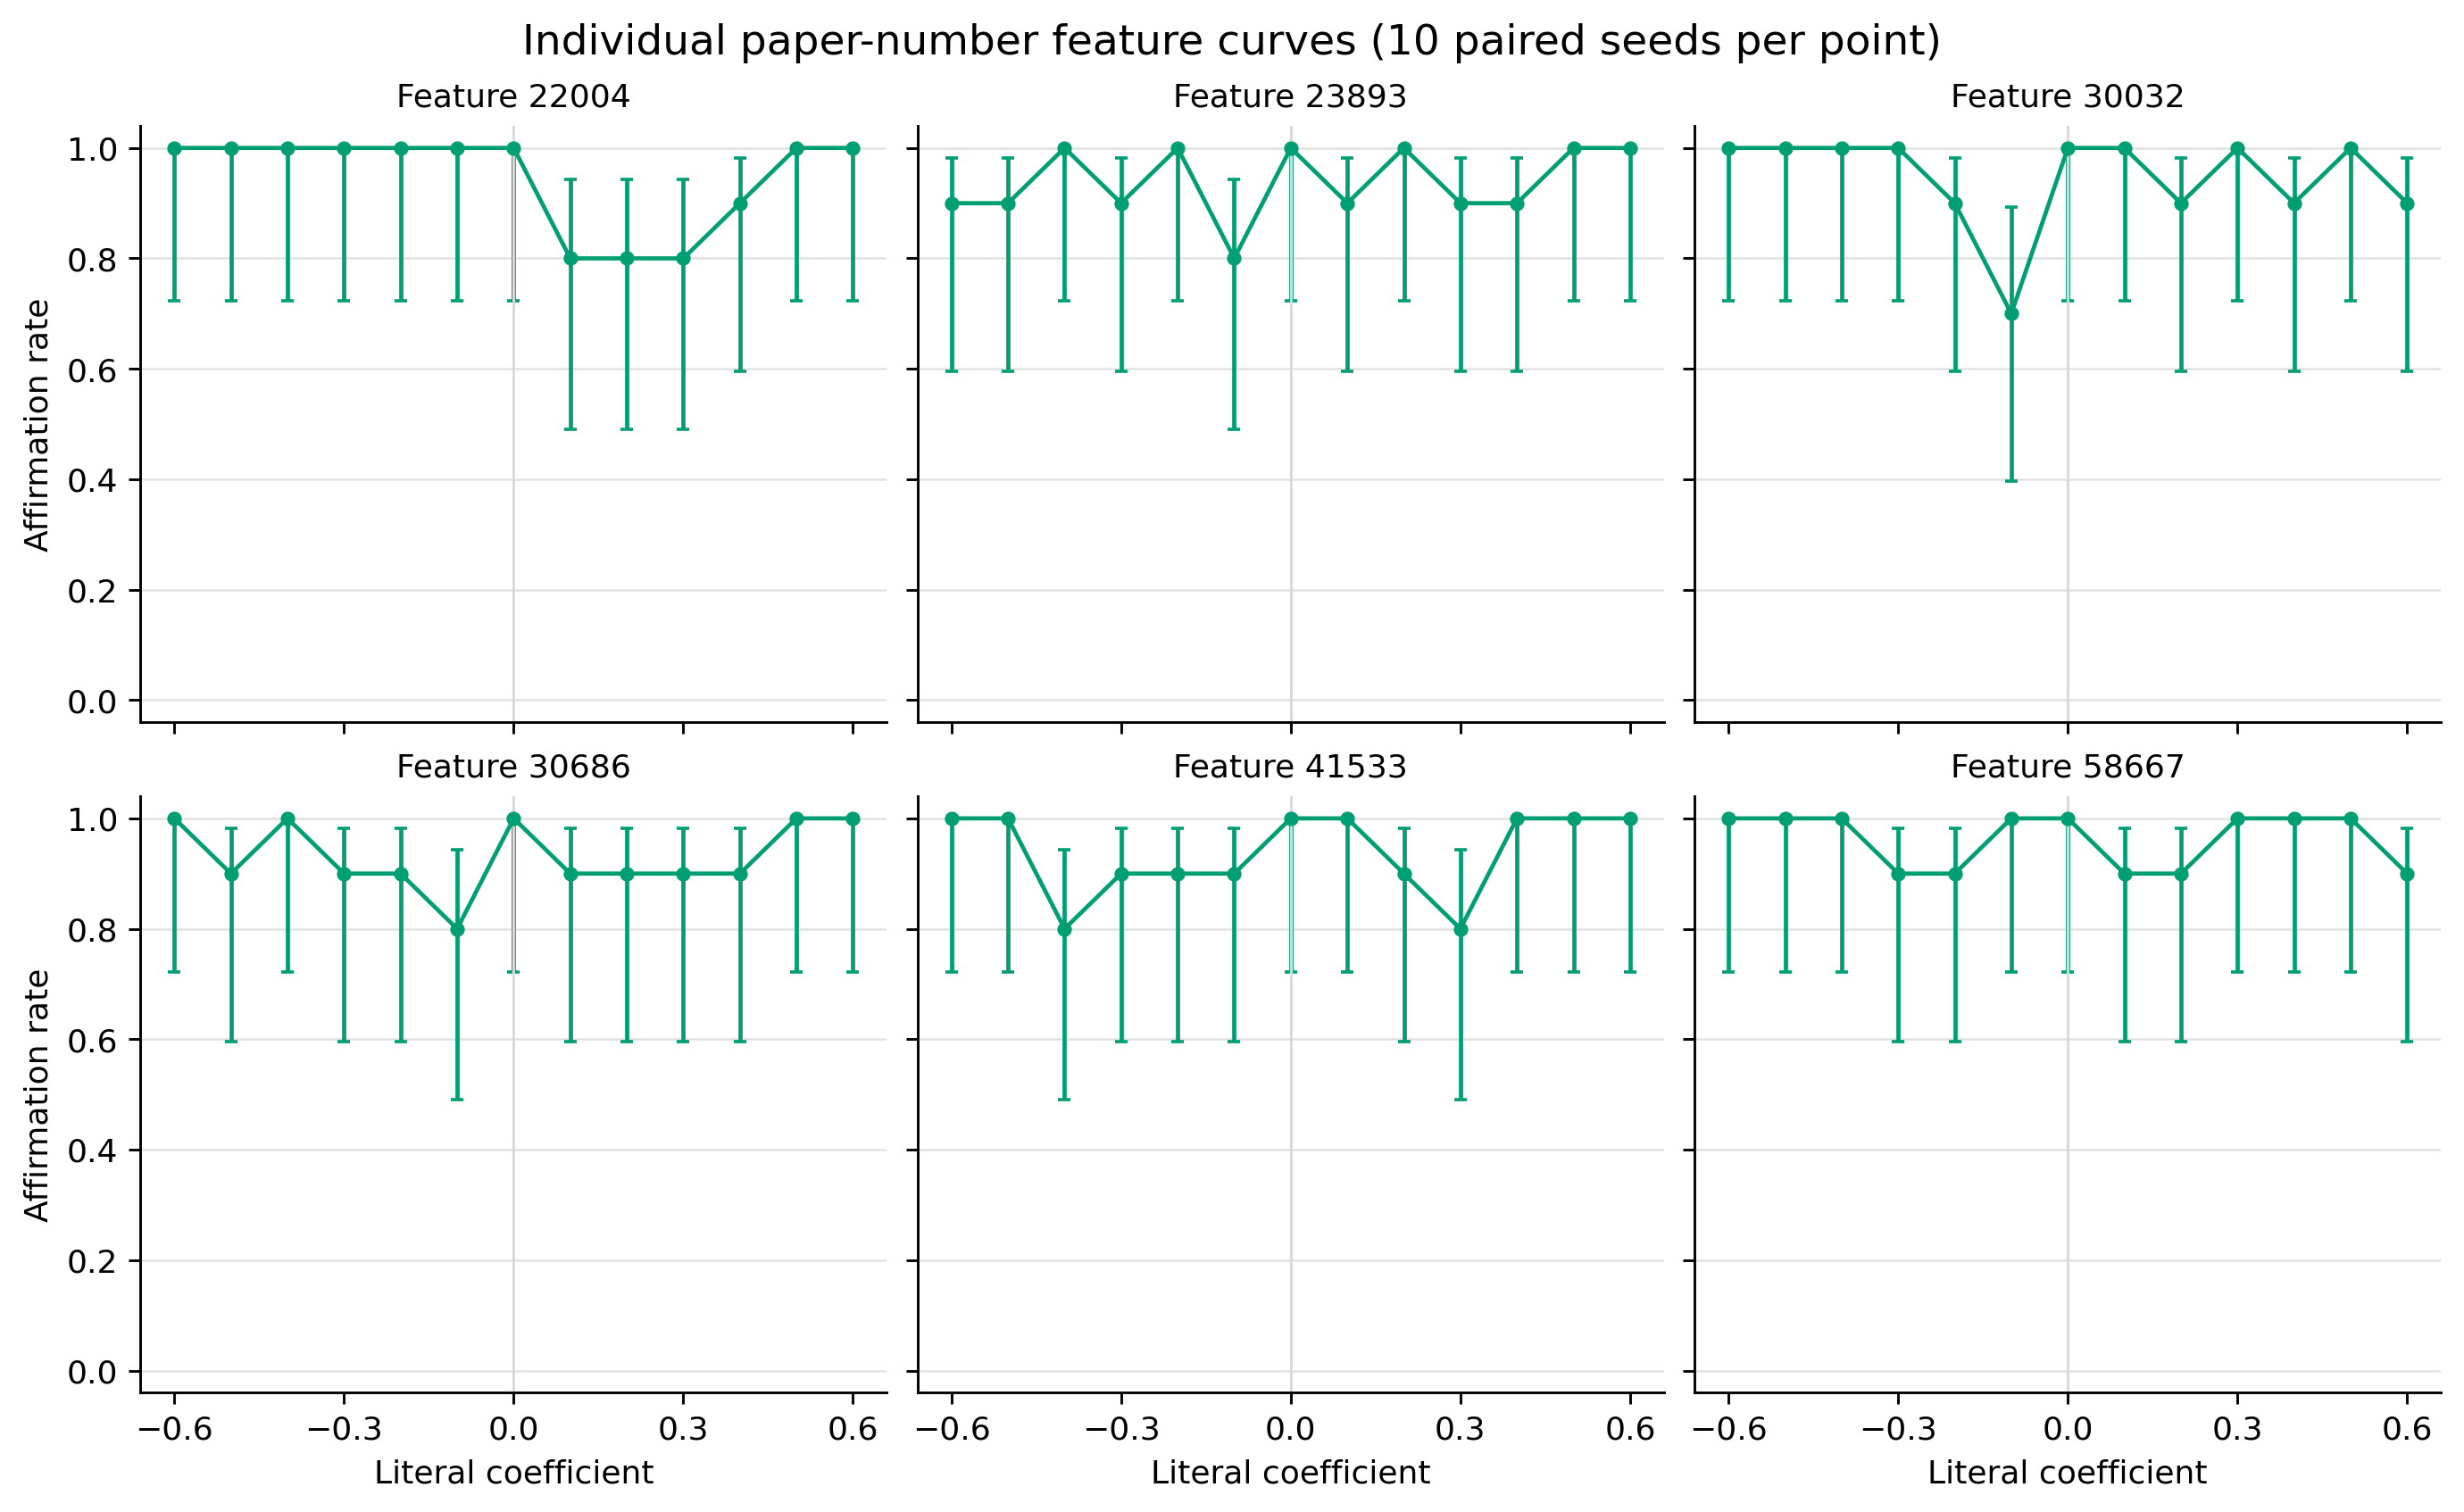
\includegraphics[width=0.99\linewidth]{results/public_sae_gating_individual_feature_curves.png}
\caption{All six prospectively frozen literal-scale individual curves, with 10 paired seeds per coefficient and 95\% Wilson intervals. Affirmation remains near ceiling and the curves are weak or nonmonotonic; no slope survives Holm correction across six features.}
\label{fig:sae-confirmatory-individual}
\end{figure}

\begin{figure}[H]
\centering
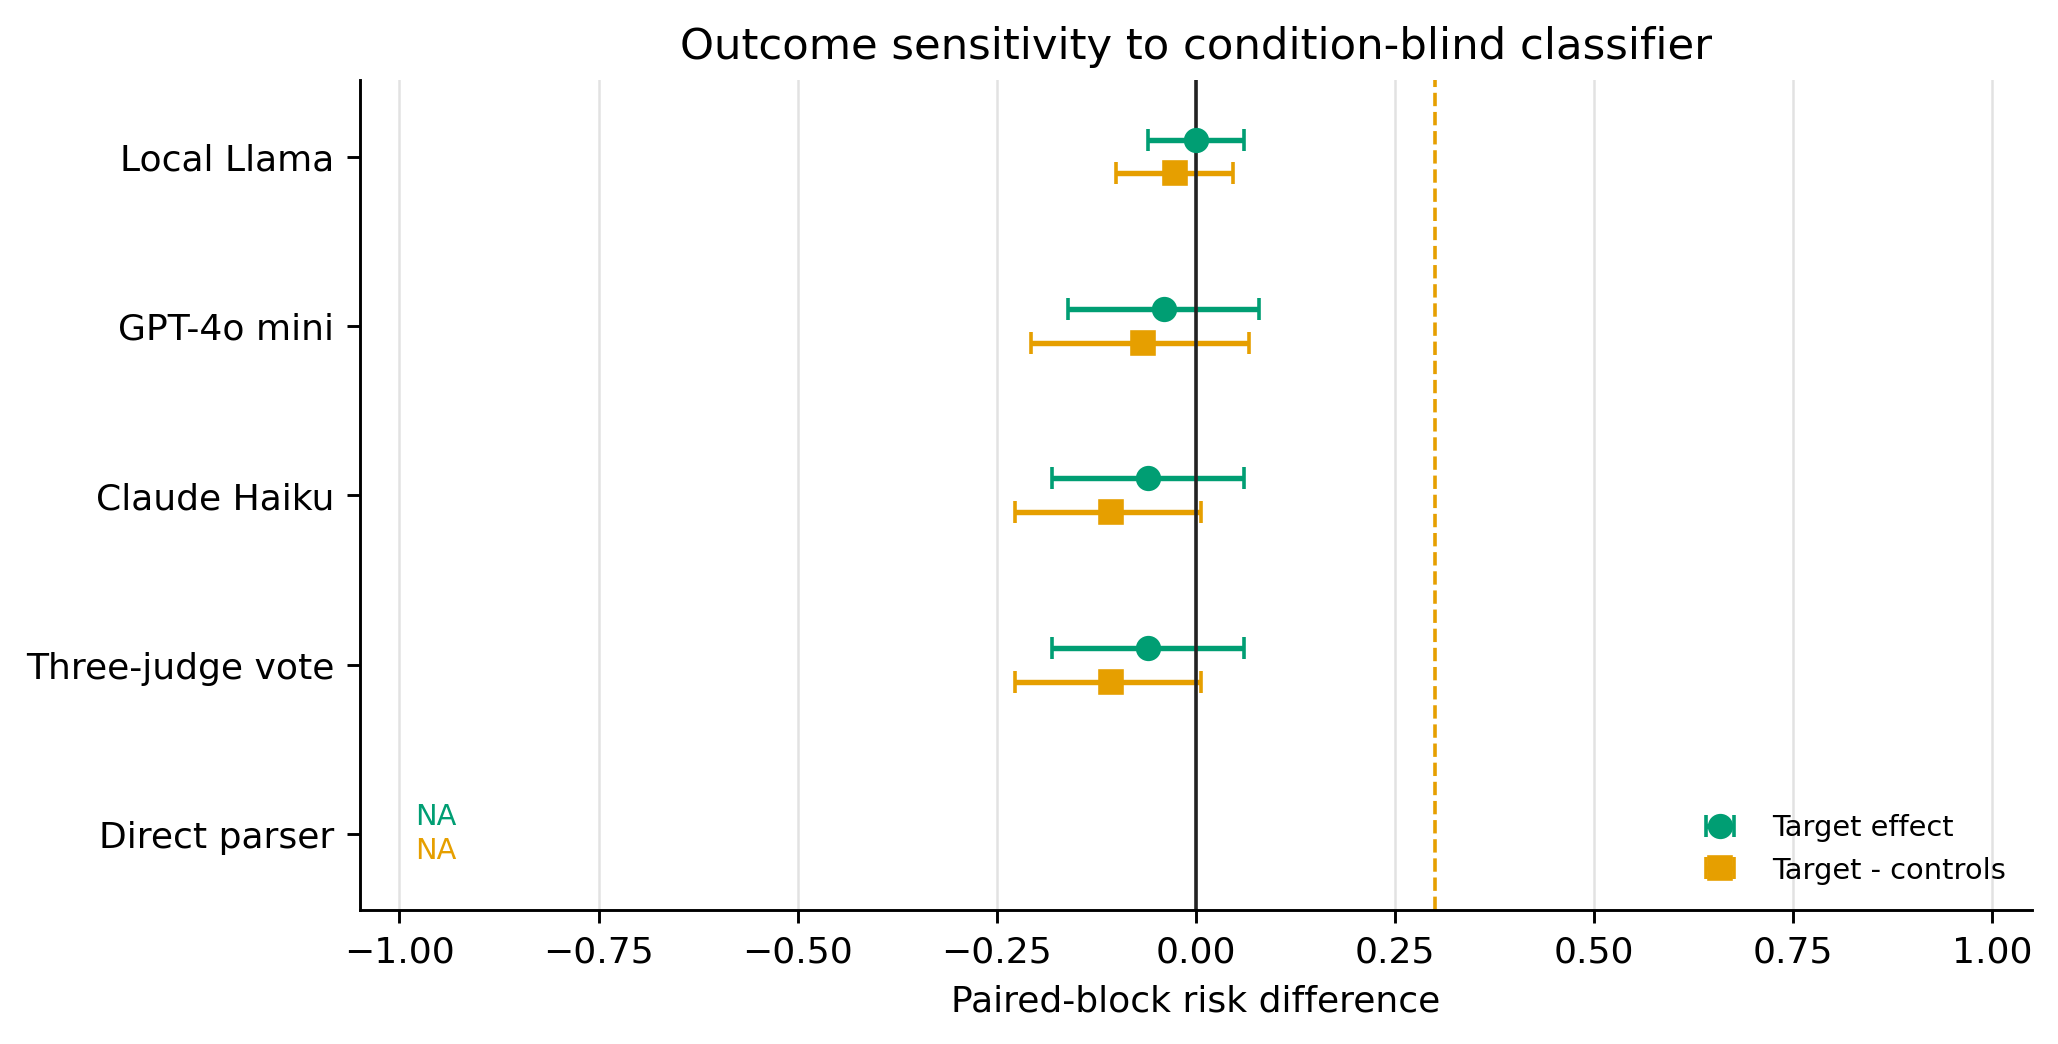
\includegraphics[width=0.92\linewidth]{results/public_sae_gating_judge_sensitivity.png}
\caption{Condition-blind outcome sensitivity. Target and target-minus-controls effects remain nonpositive or near zero under local Llama, GPT-4o mini, Claude Haiku, and three-judge majority. The strict direct parser classifies one response and has no complete paired block, so both estimates are missing.}
\label{fig:sae-confirmatory-judges}
\end{figure}

\begin{figure}[H]
\centering
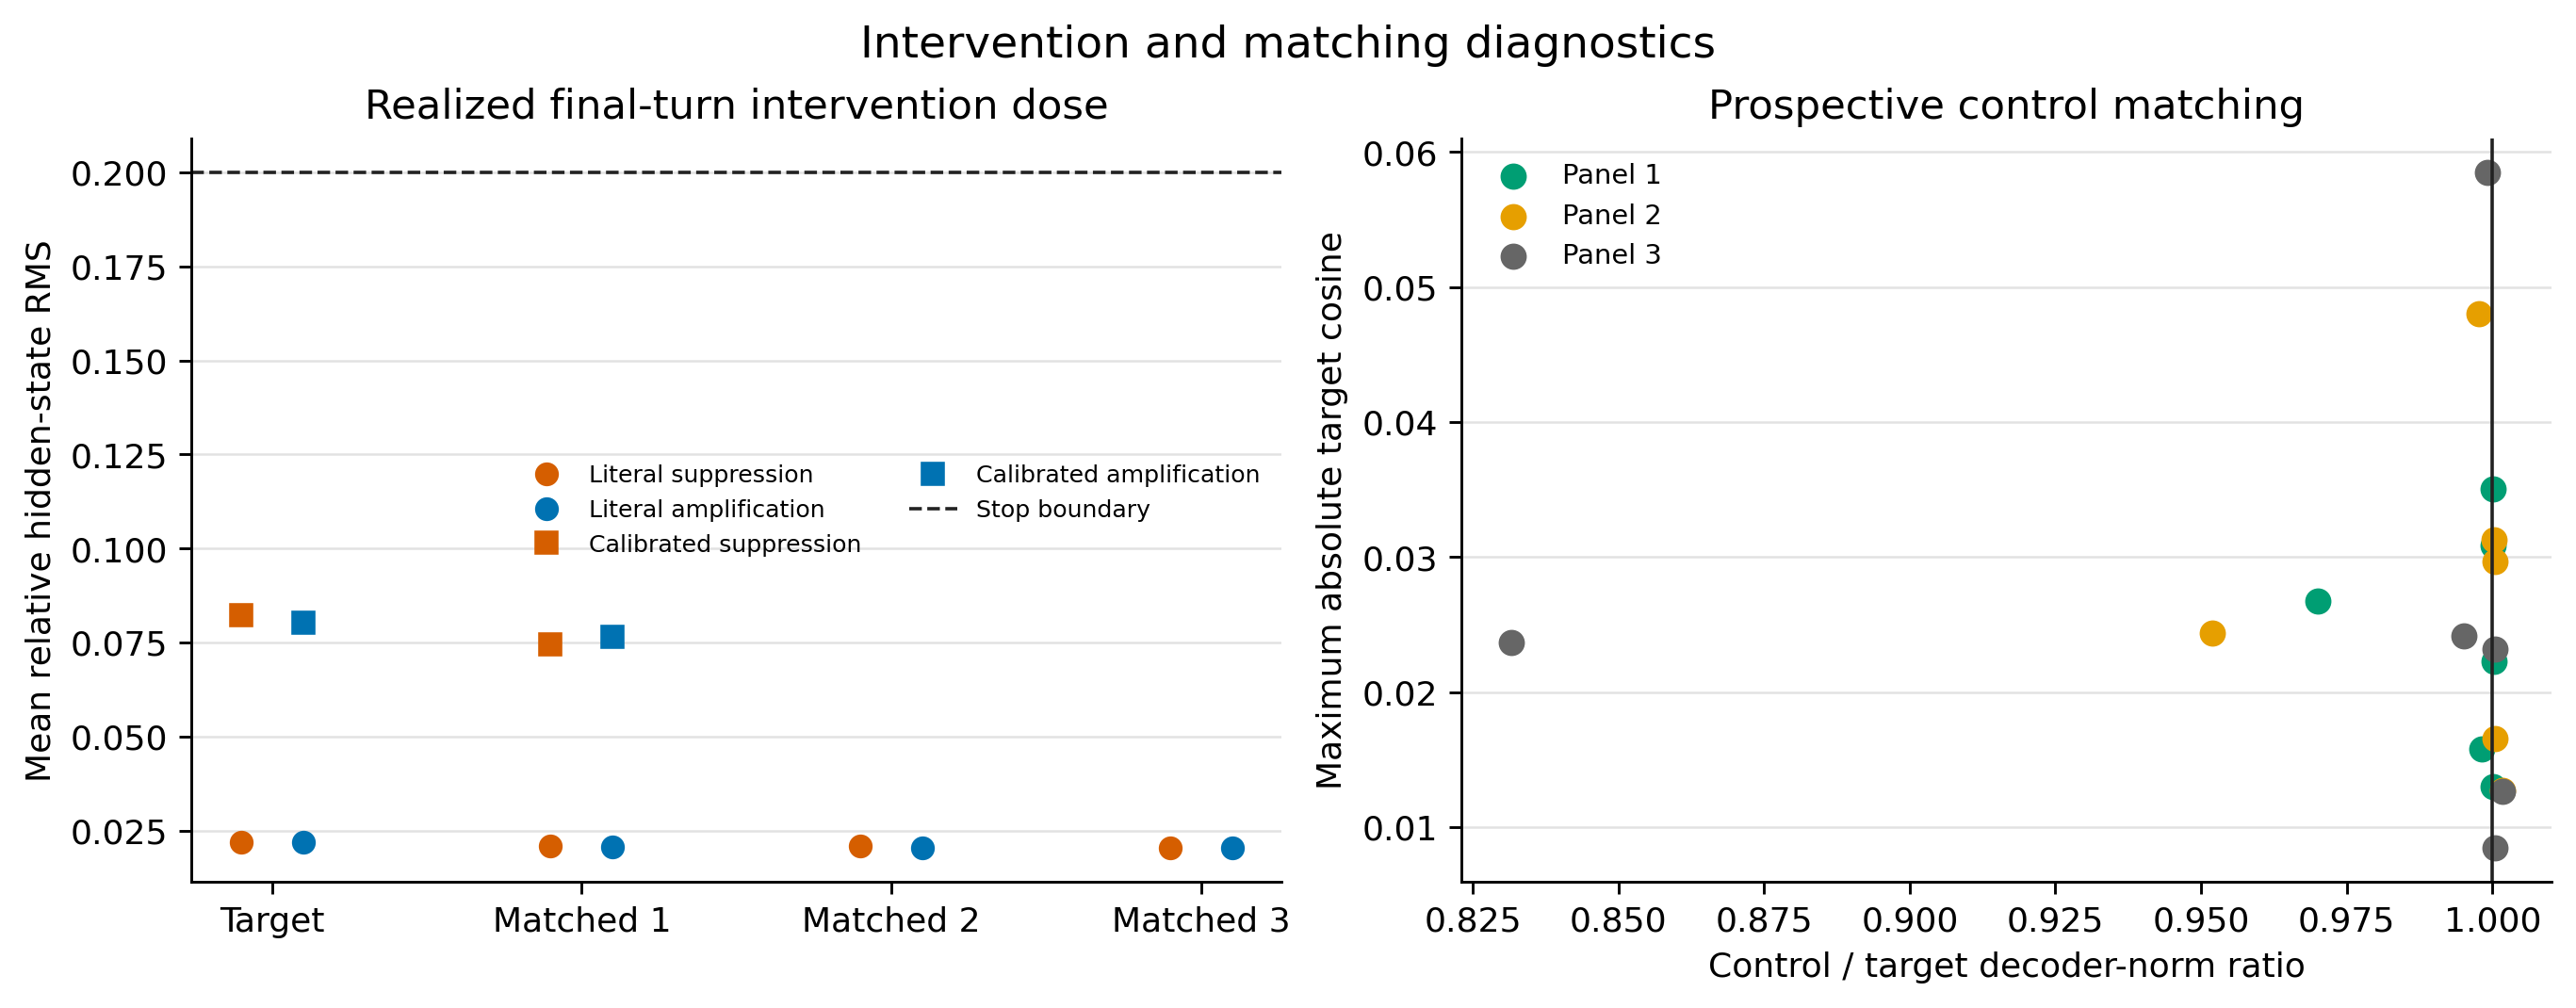
\includegraphics[width=0.98\linewidth]{results/public_sae_gating_technical_dose_and_matching.png}
\caption{Technical diagnostics for the prospective full grid. Left: realized final-turn relative hidden-state RMS by role, sign, and scale; all values remain below the 0.20 stop boundary. Right: the 18 disjoint controls satisfy the prospective decoder-norm and target-cosine calipers.}
\label{fig:sae-confirmatory-technical}
\end{figure}

\section{Gemma Scope Cross-Model Diagnostics}
\label{app:gemma}

\begin{table}[H]
\centering
\caption{Gemma Scope primary local-judge effects. Positive values follow the target paper's suppression-minus-amplification direction. Intervals are paired-block bootstrap intervals; the target-minus-controls row aligns all four roles by common block ID.}
\small
\begin{tabular}{lcc}
\toprule
Role or contrast & Effect & 95\% interval \\
\midrule
Exact self-reference $-$ history baseline & 0.12 & [0.04, 0.22] \\
Deception/roleplay target & $-0.02$ & [${-0.10},0.06$] \\
Subjective-self-report comparator & $-0.04$ & [${-0.16},0.06$] \\
Hedging/refusal comparator & 0.16 & [0.04, 0.30] \\
Matched control panel 1 & 0.00 & [${-0.12},0.12$] \\
Matched control panel 2 & $-0.06$ & [${-0.18},0.06$] \\
Matched control panel 3 & 0.04 & [${-0.12},0.20$] \\
Target $-$ mean controls & $-0.013$ & [${-0.107},0.073$] \\
\bottomrule
\end{tabular}
\end{table}

\begin{figure}[H]
\centering
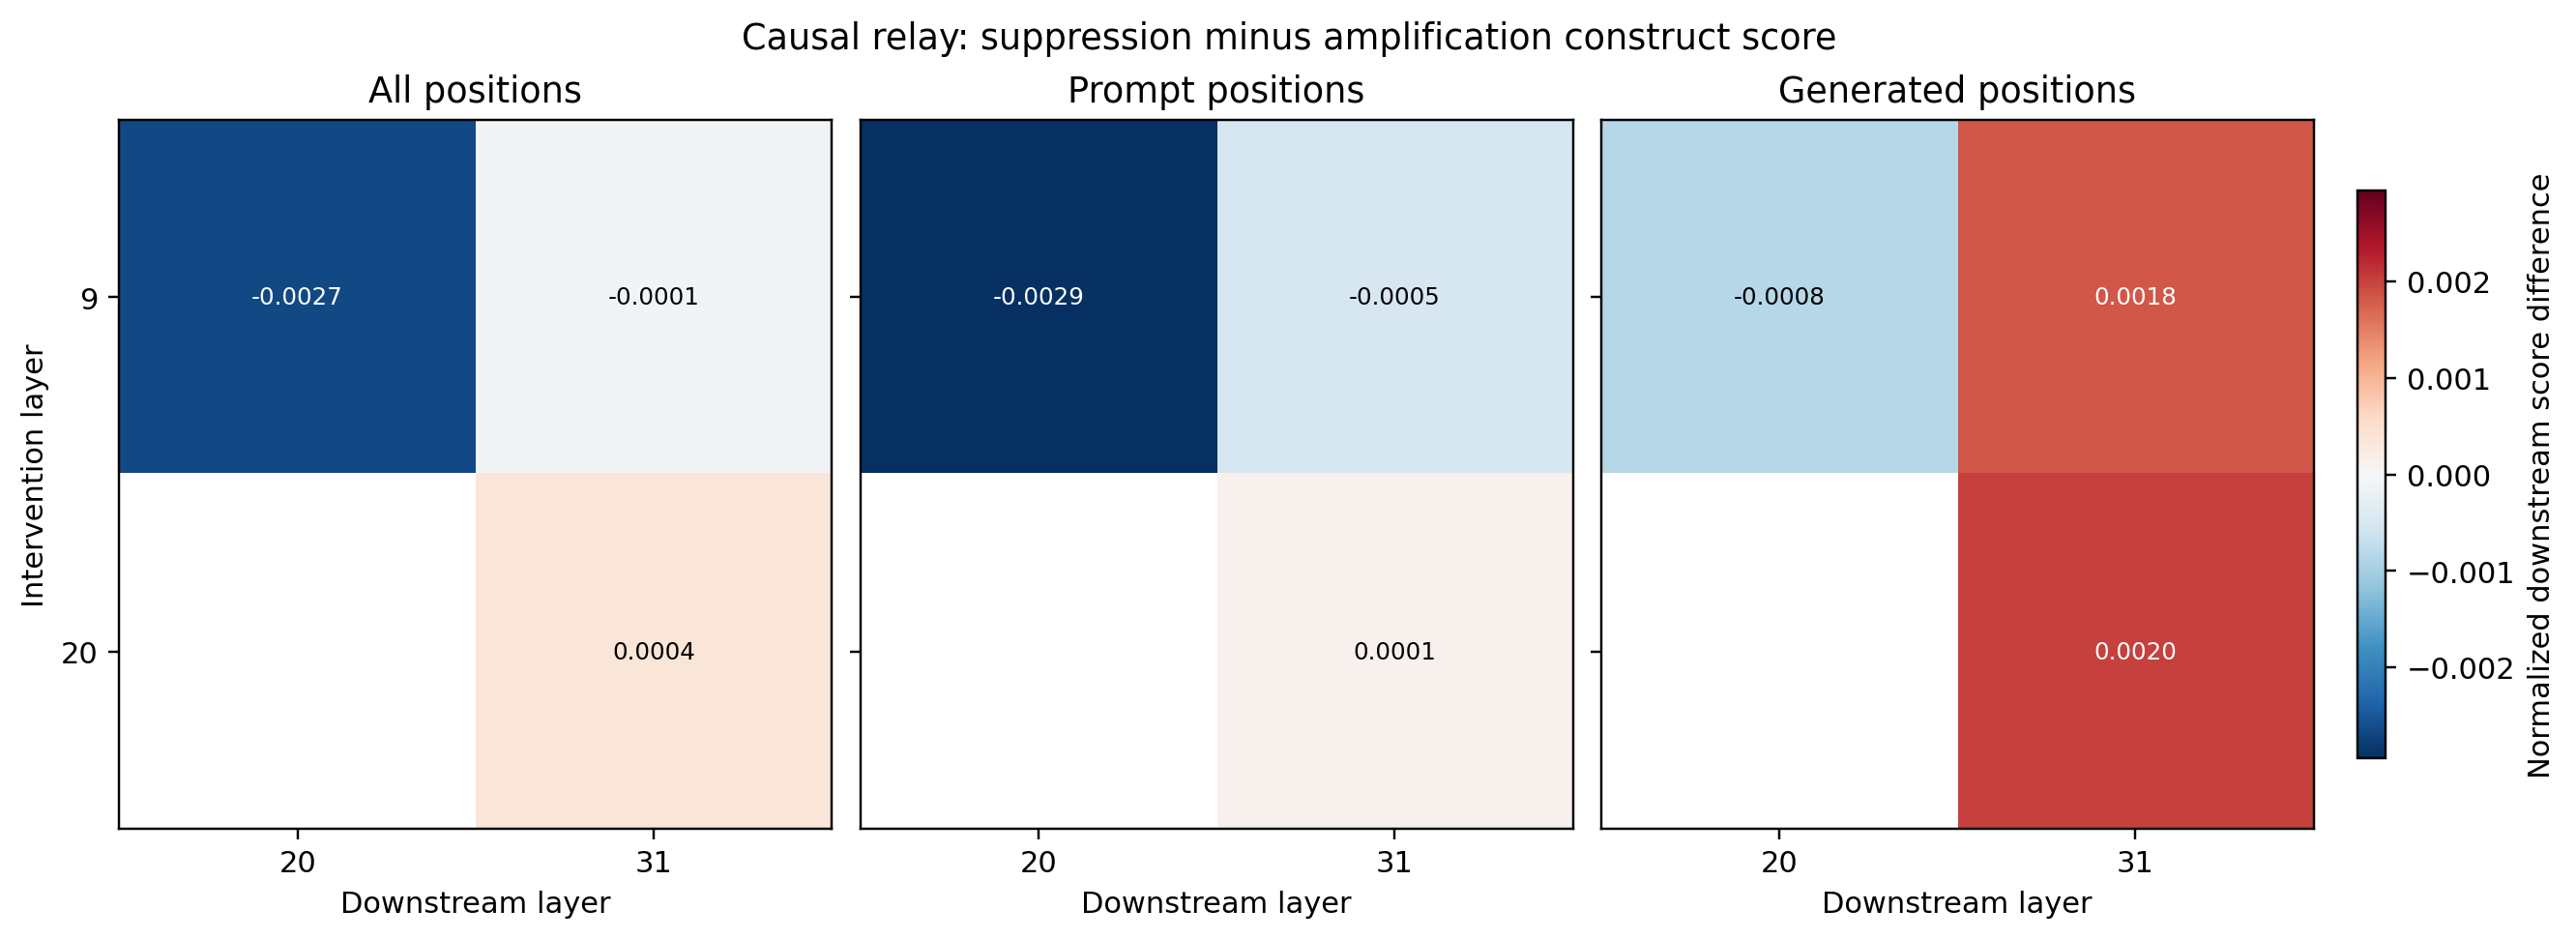
\includegraphics[width=0.99\linewidth]{results/gemma_causal_relay.png}
\caption{Direct-IT Gemma causal-relay telemetry for deception/roleplay interventions. Cells show suppression-minus-amplification differences in independently selected downstream construct scores. Layer-9-to-20 propagation has the expected negative sign and is concentrated on prompt positions; later layer-31 readouts attenuate or change sign. Blank cells are undefined same-layer or upstream readouts.}
\label{fig:gemma-relay}
\end{figure}

\begin{figure}[H]
\centering
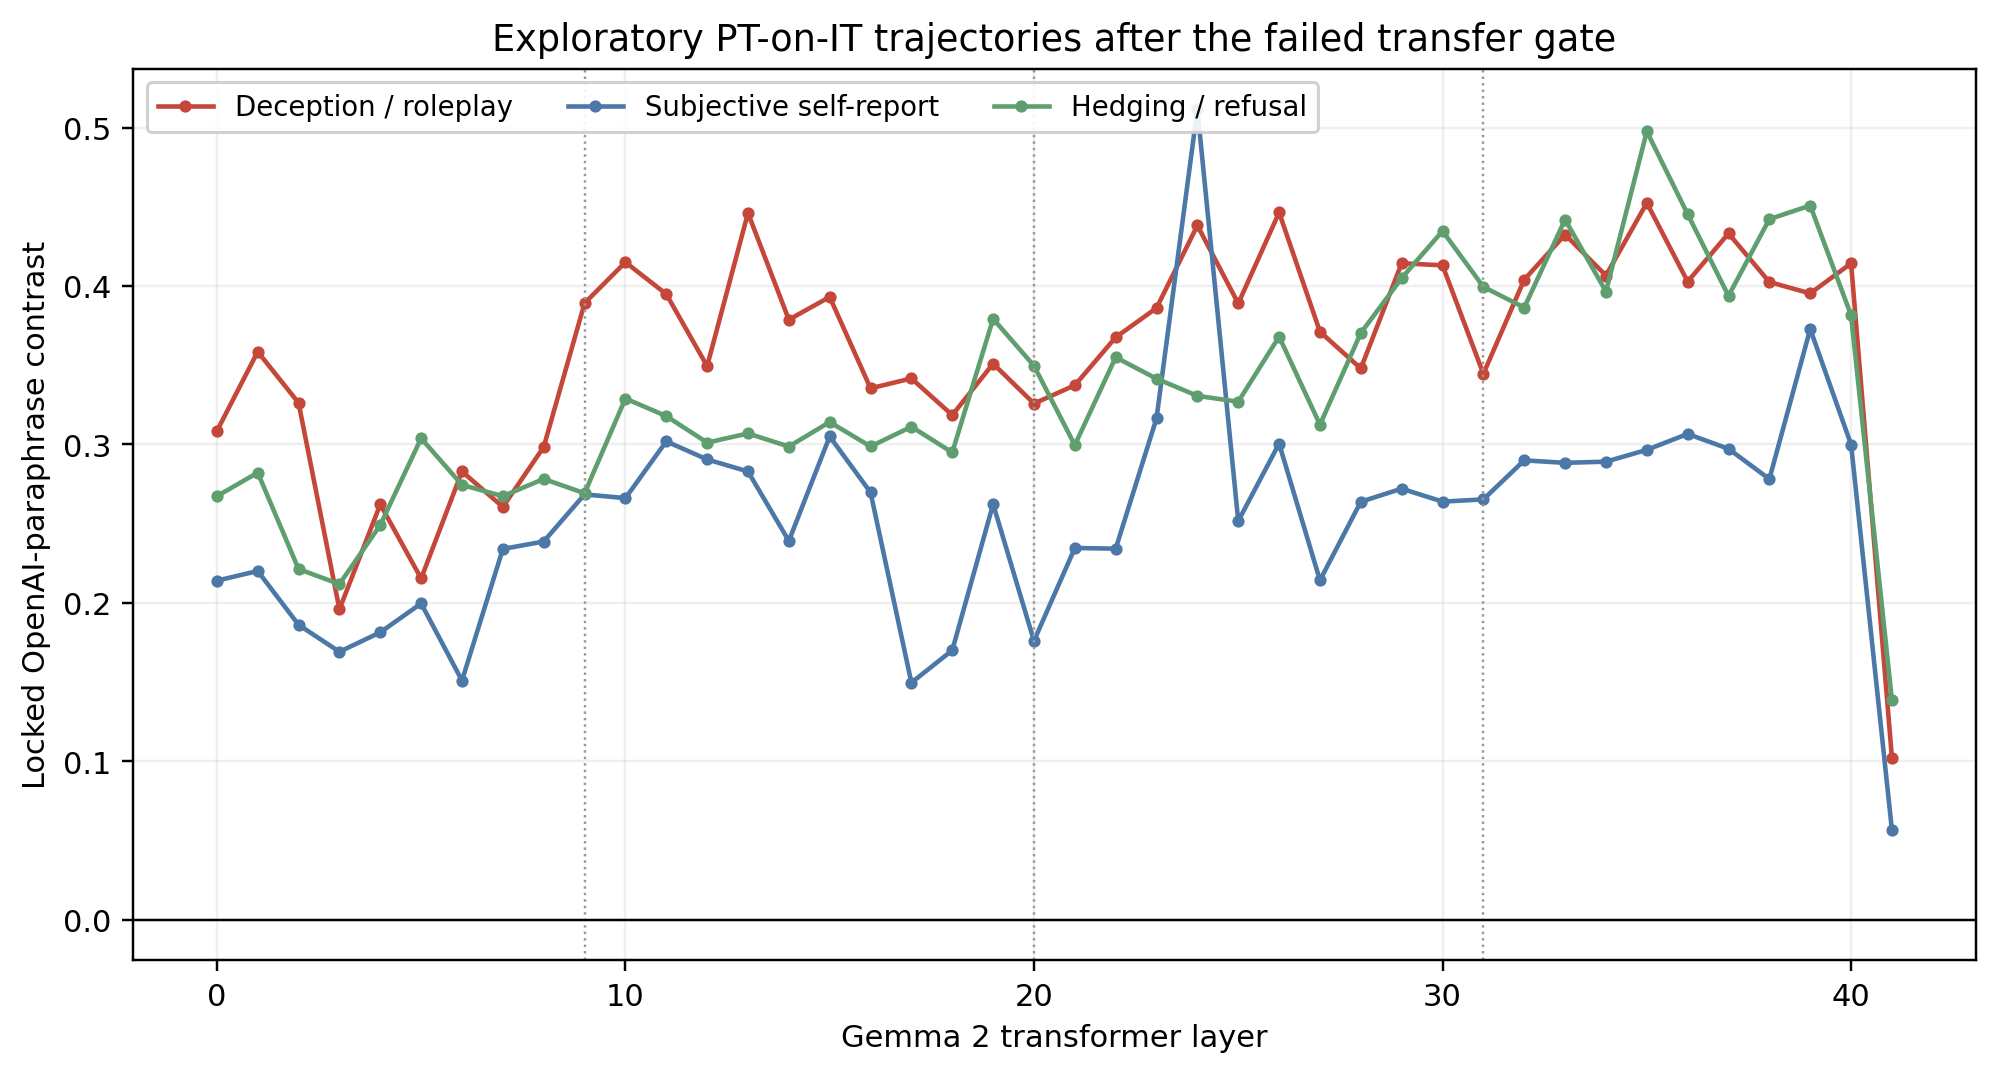
\includegraphics[width=0.99\linewidth]{results/gemma_exploratory_layerwise_construct_trajectories.png}
\caption{Exploratory 42-layer PT-SAE-on-IT construct trajectories after the prospective transfer gate failed. Every point uses six features selected independently within that layer and evaluated on locked OpenAI paraphrases. Equal feature IDs are not traced across dictionaries. Dotted lines mark direct-IT anchors. These descriptive trajectories cannot alter the direct-IT causal verdict.}
\label{fig:gemma-atlas}
\end{figure}

\section{Released Artifacts}

\begin{table}[H]
\centering
\caption{Primary causal, Llama public-SAE, and Gemma Scope release inventory.}
\small
\begin{tabular}{lr}
\toprule
Artifact & Rows \\
\midrule
Induction continuations & 480 \\
Final outcomes & 2,560 \\
Paper-style judgments & 5,120 \\
Construct-separated judgments & 5,120 \\
Complete-block human packet (v3 wave 1) & 160 \\
Public-SAE full-grid generations & 1,500 \\
Public-SAE primary judgments & 1,500 \\
Public-SAE external judgments & 3,000 \\
Gemma baseline generations & 180 \\
Gemma steering generations & 830 \\
Gemma primary judgments & 1,010 \\
Gemma external judgments & 2,020 \\
\bottomrule
\end{tabular}
\end{table}

Every JSONL identifier is unique within its artifact. The release manifests record file hashes, four empty causal-study outcomes, the retained transient causal judge-format error, two zero-row public-SAE judge startup failures, and the fail-closed Gemma exploratory hook-mismatch correction. Private keys, Hugging Face tokens, coder linkage keys, and model caches are excluded.

\clearpage
\begingroup
\small
\bibliographystyle{plainnat}
\bibliography{references}
\endgroup

\end{document}
